\chapter{An Effective Contact Dynamics Model for Contact-rich Planning}
\label{chapter:quasi_static_dynamics}
\section{Introduction}
We believe an effective model for contact-rich manipulation planning needs to be 
(\textbf{i}) numerically robust
and (\textbf{ii}) differentiable, so that local linearizations can be reliably computed for planning. 
Most importantly, the model should be able to (\textbf{iii}) predict the \emph{long-term} behavior of the system, so that the planner can look far ahead while taking few steps.
Last but not least, the model should be (\textbf{iv}) amenable to smoothing in order to provide more informative locally linear models across contact modes. 

In this chapter, we present a contact dynamics model that satisfies all of the requirements above. Combining these ingredients enables our planner to reliably generate complex contact-rich plans that have so far been considered challenging for existing model-based approaches.

Specifically, we propose a \emph{convex} implicit time-stepping contact model (Sec. \ref{sec:convex_quasi_dynamic_contact_dynamics}). 
Among several existing schemes to convexify frictional contact constraints (Sec. \ref{sec:quasi_static_background}), we adopt Anitescu's convex relaxation \cite{anitescu2006optimization} which in practice only introduces mild non-physical behavior \cite{pang2021convex, castro2021unconstrained}. The convexity provides a clear numerical advantage over the traditional Linear Complementarity Problem (LCP) formulation \cite{anitescu1997formulating, stewart2000rigid}. Moreover, the derivatives of the dynamics with respect to the current state and control action can be readily computed using sensitivity analysis for convex conic programs \cite{agrawal2019differentiatingcone} (Sec. \ref{sec:quasi_dynamic_derivatives}). In addition, we will illustrate how Anitescu's convex relaxation compares to the LCP formulation, and why it introduces a non-physical ``boundary layer'' during sliding (Sec. \ref{sec:quasi_static:artifacts}).

For long-term predictability, we adopt the quasi-static assumption widely used in robotic manipulation \cite{mason2001mechanics, motioncones, aceituno2020global, cheng2021contact}. 
A quasi-static model ``sees'' further than its second-order counterpart by ignoring transient dynamics and focuses on transitions between steady-states. Furthermore, quasi-static models are simpler: not only do they have half as many states, they also do not need parameters to describe damping, as damping is modeled by throwing away kinetic energy at every time step.

In our quasi-static model, robots are modeled as an impedance source. However, throughout the long history of quasi-static models in robotic manipulation planning (Sec. \ref{sec:quasi_static_background}), robots have often been modeled as an admittance source. This can lead to an ill-defined behavior where the output cannot be uniquely determined by the input, thereby limiting the utility of quasi-static models in contact-rich planning. In Sec. \ref{sec:quasi_static:prescribed_motion_bad}, we will elaborate on the limitations of the admittance modeling choice, and how impedance can resolve these problems.

The proposed quasi-static model is validated by running the same input trajectories in a high-fidelity second-order simulator (Sec. \ref{sec:quasi_static:experiments}). Our results show that our model is able to approximate the second-order dynamics well if the system considered is highly damped and dominated by frictional forces. Furthermore, in contact-rich scenarios, our model can keep the simulation error small at larger step sizes than the second-order simulator.
 
Lastly, to leverage the benefits of smoothing (Sec. \ref{sec:smoothdynamics}) in contact-rich planning, we show that in addition to the standard randomized smoothing schemes (Sec. \ref{sec:randomizedmoothing}), our contact model can be smoothed out using a log-barrier relaxation (Sec. \ref{sec:analyticsmoothing}). In this relaxation scheme, the hard contact constraints are softly enforced by a log-barrier function, a common technique used in the interior-point method for convex programs \cite[\textsection 11]{boyd2004convex} \cite{howell2022dojo}.
We further show that the gradients of the smoothed contact model can be easily computed with the implicit function theorem.


\section{Background} \label{sec:q_dynamics:background}
In this section, we will review how quasi-static dynamical models have been applied in manipulation planning, and highlight the flaw of modeling robots as an admittance source (Sec. \ref{sec:quasi_static_background}). We will also discuss the features of and trade-offs between various convex relaxations of rigid-body contact models (Sec. \ref{sec:convex_contact_background}).

\subsection{Quasi-static Models in Robotic Manipulation} \label{sec:quasi_static_background}
Quasi-static models, which previous works have used extensively for robotic manipulation planning and control \cite{mason2001mechanics, motioncones, aceituno2020global, cheng2021contact, pang2021easing}, simplify Newtonian dynamics by removing terms related to velocity and acceleration, and focusing on contact forces at the core of robot-object interactions. Although the model cannot describe highly-dynamics behaviors such as spinning a pen between fingers \cite{mordatch2012contact}, it holds up for a wide variety of manipulation tasks, including many that involve dexterous hands \cite{andrychowicz2020learning}.

Quasi-static models also have a long history in robotic manipulation. Planar pushing is perhaps one of the earliest problems where quasi-static models are applied. Pioneering work by Mason and Lynch focuses on predicting the motion of an object supported on a horizontal surface without knowledge of the pressure distribution between the object and the surface \cite{mason1986mechanics, lynch1996stable}. Later work incorporates a detailed pressure distribution \cite{goyal1991planar, howe1996practical} and stochasticity \cite{zhou2017fast} into the quasi-static planar pushing model. Such models have been effectively employed in a Model Predictive Control (MPC) framework which enables an object pushed by a single point contact to track complex planar trajectories \cite{hogan2020feedback}. In addition to planar pushing, quasi-static models have also been applied in simple, planar instances of dexterous manipulation \cite{trinkle1993dexterous, pang1996complementarity}.

Halving the number of states by removing velocity is one of the most recognized advantages of quasi-static systems \cite[\textsection 10.1]{mason2001mechanics}.
However, by focusing on transitions between static equilibria and ignoring transients induced by damping and acceleration, a quasi-static model can look further into the future while taking fewer steps than its second-order counterpart, thereby reducing the planning horizon. 
We believe this temporal aspect of quasi-static models' advantage is important but often overlooked in the literature. In practice, many trajectory optimization formulations for manipulation enforce the second-order Newtonian dynamics \cite{landry2019differentiable, kurtz2022contact}. Although modeling the transients allows the discovery of more dynamic behaviors, we believe, especially in the manipulation setting, that the added computational complexity due to long planning horizon oftentimes outweighs the benefits. 

Despite their popularity, many popular variants of quasi-static models, such as \cite{mason1986mechanics, lynch1996stable, zhou2017fast, hogan2020feedback}, have a serious flaw: the next state cannot be always be uniquely determined from the current state and control input.
In quasi-static models, the control input is usually defined as the position commands of the robots. 
Many quasi-static models also assume that the position commands can be perfectly executed as prescribed robot motions. Under this assumption, contact forces and object motions can be ambiguous for the same control input. This flaw does not manifest in simple tasks such as planar pushing, where robot motion does uniquely determine object motion. On the other hand, it can be crippling in more complex tasks such as grasping (more details in Sec. \ref{sec:quasi_static:prescribed_motion_bad}). 

It is possible to circumvent the ambiguity by including contact forces as additional states of the dynamics model \cite{trinkle1993dexterous, aydinoglu2020contact}. However, reasoning about both positions and forces compels the planner to handle the complementarity constraints between forces and distances, thereby limiting the algorithms the planner can employ.

A more fundamental remedy to this flaw is to account for the unmodeled compliance in the system, thereby allowing commanded and actual robot positions to be different. For instance, Harm and Posa added compliance at the robot joints by modeling the robot as velocity-controlled with finite gains \cite{halm2018quasi}; in previous work we added compliance at the contact points \cite{pang2018robust}. However, these remedies do not always reflect the reality on robotic hardware, which often consists of rigid objects and impedance-controlled robots. Moreover, \cite{pang2018robust} is too computationally expensive, and \cite{halm2018quasi} is developed specifically for manipulating planar objects supported on a tabletop.

In Sec. \ref{sec:quasi_static:prescribed_motion_bad}, we will discuss in more detail the flaws of commanding prescribed robot motions, and how our quasi-static formulation resolves it in a computationally-efficient and hardware-consistent manner. 


\subsection{Convex Rigid-body Contact Dynamics} \label{sec:convex_contact_background}
Without friction, quasi-static dynamics with frictionless unilateral contacts can be written as the KKT optimality conditions of a convex Quadratic Program (QP) that minimizes the system's potential energy subject to non-penetration constraints \cite{pang2021convex}. The complementarity between forces and distances (Sec \ref{sec:intro:complementarity_constraints}) are captured by the complementarity slackness between primal constraints and dual variables. However, the Coulomb friction law and the maximum dissipation principle, both of which are needed to model frictional contacts, introduce additional complementarity constraints that can no longer be accommodated by a convex program. Consequently, contact dynamics with Coulomb friction is formulated as an LCP, which is solved by specialized non-convex solvers \cite{anitescu1997formulating, stewart2000rigid}.

Anitescu restored convexity in contact dynamics by replacing the linear complementarity constraints with cone complementarity constraints. The price of convexity is that the sliding velocity is no longer restricted to the tangent plane defined by the contact normal \cite{anitescu2006optimization, SiggraphContact22}. The resulting program is a convex QP with discretized friction cones, or a Second-Order Cone Program (SOCP) with circular friction cones. Both formulations can be readily solved with commercial convex solvers such as \cite{mosek}.

Anitescu's convex relaxation exactly reproduces Coulomb friction when the contact is sticking, and injects a non-physical ``boundary layer'' between relatively-sliding objects. A big advantage of Anitescu's relaxation is that the extent of relaxation is controlled by only one hyperparameter: the step size. As the step size converges to 0, the boundary layer also vanishes \cite{anitescu2006optimization}. The step size therefore can serve as a knob that allows the planner to trade the dynamics model's predictive power for physical accuracy. We will discuss this non-physical behavior in more detail in Sec. \ref{sec:quasi_static:artifacts}.

The popular MuJoCo simulator\cite{todorov2012mujoco, todorov2014convex} solves a convex program that closely resembles the dual of Anitescu's formulation \cite[Appendix B]{underactuated}. Moreover, Mujoco also adds regularization on contact forces to the objective function in order to improve numerical conditioning and make the dynamics invertible. However, the regularization introduces non-physical behaviors such as ``force at a distance'' that are harder to control as they are induced by many hyper-parameters \cite{kolbert2016experimental}. 

Recently, Castro \textit{et al.} developed an unconstrained convex formulation of contact dynamics \cite{castro2021unconstrained} that combines many of the nice features from MuJoCo \cite{todorov2012mujoco} and Anitescu's convex relaxation \cite{anitescu2006optimization}. For instance, Castro's primal formulation is similar to Anitescu's; the contact force regularization and the removal of friction cone constraints using a projection function are inspired by similar techniques from MuJoCo. 
Castro's formulation is designed from ground up for efficient and accurate physics simulation. For instance, it provides physical interpretations and units to the contact force regularization parameters that are originally proposed by MuJoCo to improve numerical conditioning.
% Similar to MuJoCo, Castro's unconstrained formulation has regularization on contact forces. However, Castro proposed a rigorous methodology for setting the regularization in a way that respects simulation accuracy. 


\section{A Convex, Quasi-static and Differentiable Contact Model} \label{sec:q_dynamics:cqdc}
In this section, we present the Convex, Quasi-static, Differentiable Contact (CQDC) model which will be used for the contact-rich planning tasks in Chapter \ref{chapter:contact_rich_planning}. Specifically, we will start with the equations of motion of quasi-static contact dynamics, and massage it into the KKT optimality conditions of a convex optimization program (Sec. \ref{sec:convex_quasi_dynamic_contact_dynamics}). We will then describe how to take the (discontinuous) derivatives of the proposed contact dynamics (Sec. \ref{sec:quasi_dynamic_derivatives}), and how the forward dynamics and gradient computation are implemented (Sec. \ref{sec:quasi_static:implementation}). In addition, we will illustrate how Anitescu's convex relaxation introduces a non-physical ``boundary layer'' during sliding (Sec. \ref{sec:quasi_static:artifacts}). We will also dive more deeply into the common flaw in quasi-static dynamical models brought up in Sec. \ref{sec:q_dynamics:background}, and explain how our quasi-static model resolves it (Sec. \ref{sec:quasi_static:prescribed_motion_bad}). Lastly, with two examples of common manipulation tasks, we show that the proposed quasi-static model and an established second-order simulator (Drake \cite{drake}) generate very similar state trajectories for the same action sequence (Sec. \ref{sec:quasi_static:experiments}). 

\subsection{Forward Dynamics} \label{sec:convex_quasi_dynamic_contact_dynamics}
Despite the numerical advantage of convex contact dynamics formulations \cite{anitescu2006optimization, todorov2012mujoco, castro2021unconstrained}, some formulations can produce highly inaccurate contact forces with poorly-chosen hyperparameters \cite{kolbert2016experimental}. Our formulation adopts Anitescu's convex relaxation of the Coulomb friction constraints \cite{anitescu2006optimization}. Anitescu's convex relaxation is equivalent to common LCP formulations \cite{stewart2000rigid} in non-sliding contacts or in separation, and introduces a non-physical yet mild ``boundary layer'' effect between relatively-sliding objects \cite{pang2021convex, castro2021unconstrained}. Not only does Anitescu's convex friction model have the simulation step size $h$ as the only hyperparameter, the ``boundary layer'' also disappears as $h \rightarrow 0$. The step size therefore can serve as a knob that allows the planner to trade the dynamics model's predictive power for physical accuracy.

A generic discrete-time dynamical system is written as
\begin{equation}
\label{eq:f_x_u}
x_+ = f(x, u) 
\end{equation}
where $x \in \mathbb{R}^n$ is the state, $u \in \mathbb{R}^m$ the control input, and $f: \mathbb{R}^n\times\mathbb{R}^m\rightarrow\mathbb{R}^n$ the system dynamics. 
In the robotic manipulation setting, a system can be divided into $\nA$ \emph{actuated} Degree of Freedoms (DOFs), which correspond to the robots, and $\nU$ \emph{unactuated} DOFs, which correspond to the objects. The configurations of objects and robots are denoted respectively by $\qu \in \R[\nU]$ and $\qa \in \R[\nA]$. The system state is defined by $x \coloneqq q \coloneqq (\qu, \qa)$. We model the robots as impedances \cite{hogan1985impedance}, which in the quasi-static setting reduces to springs with a diagonal stiffness matrix $\Ka \in \R[\nA \times \nA]$. Accordingly, the input $u \in \R[\nA]$ is defined by the commanded positions of the robots' joints, which can also be interpreted as the equilibrium positions of the springs.

The discretized quasi-static equations of motion are
\begin{subequations}
\label{eq:q_dynamics_eom}
\begin{align} 
h \Ka \left(\qa + \dqa - u \right) &= h\tauA + \sum_{i=1}^{\nC} (\Ja[i])^\intercal \lambda_i, \label{eq:q_dynamics_eom:a}\\
\left( \frac{\epsilon}{h} \Mu \right) \dqu &= h\tauU + \sum_{i=1}^{\nC} (\Ju[i])^\intercal \lambda_i, \label{eq:q_dynamics_eom:u}
\end{align}
\end{subequations}
where $h \in \R_{++}$ is the step size in seconds; $\Mu \in \R[\nU \times \nU]$ is the mass matrix of the objects; $\epsilon \in \R_{+}$ is a small regularization constant; the change in system configuration from the current to the next step is $\dq \coloneqq (\dqu, \dqa)$; $\tauA \in \R[\nA]$ and $\tauU \in \R[\nU]$ are non-contact external torques (e.g. due to gravity) for robots and objects. There are $\nC$ contact pairs at the current time step. For the $i$-th contact, $\lambda_i \in \R[3]$ is the contact impulse; $\Ja[i] \in \R[3 \times \nA]$ and $\Ju[i] \in \R[3 \times \nU]$ are the contact Jacobians \cite{anitescu1996formulating} of the robots and the objects, respectively. For 3D systems, it is common that the rotational displacement and the angular velocity are different and related by a linear map. As the technique to deal with this difference is standard (e.g. \cite[Section II]{castro2021unconstrained}), we leave it out here for brevity and notational simplicity.

Equation \eqref{eq:q_dynamics_eom:a} states that the robot joint positions' deviation from their commanded values $u$, as a result of external impulses, is proportional to the stiffness $\Ka$. 
Equation \eqref{eq:q_dynamics_eom:u} can have different physical interpretations depending on the value of the regularization constant $\epsilon$.
If $\epsilon = 0$, \eqref{eq:q_dynamics_eom:u} is the force (impulse) balance of the objects. This corresponds to the exact quasi-static formulation in  \cite{pang2021convex}. 
If $\epsilon = 1$, \eqref{eq:q_dynamics_eom:u} is the standard second-order rigid body equations of motion (expressed in impulse-momentum form) for a system with 0 velocity at the current time step. 
This corresponds to Mason's classical definition of quasi-dynamic systems \cite{mason2001mechanics}. 
Note that for any $\epsilon$, the momentum gained at every step due to external impulses is discarded at the next time step, which is characteristic of the highly damped behavior typical in quasi-static systems.

In our physical experiments in later sections where objects are light, we find that the dynamics is closer to being exactly quasi-static ($\epsilon = 0$) than being classically quasi-dynamic ($\epsilon = 1$). Therefore, we pick $\epsilon$ to be as small as possible without causing numerical issues. A rule of thumb is to set $\epsilon$ such that the largest eigenvalue of $(\epsilon \Mu / h)$ is one tenth of the smallest eigenvalue of $(h \Ka)$ (see the definition of $\mathbf{Q}$ in \eqref{eq:q_dynamic_socp:Q_and_b}).
% $\epsilon$ needs to be set based on how much damping forces the robot experiences as it interacts with the object.

In addition, the Coulomb friction model requires the contact impulses $\lambda_i$ to stay inside the friction cone, and the relative sliding velocities to satisfy the maximum dissipation principle \cite{stewart2000rigid}. To enforce these constraints, we first introduce some additional notation. The contact Jacobian for contact $i$ is 
\begin{equation}
\label{eq:contact_jacobian_i}
\J_i \coloneqq [\Ju[i], \Ja[i]] \coloneqq 
\begin{bmatrix}
\Jn[i] \\
\Jt[i]
\end{bmatrix}
\in \R[3 \times (\nU + \nA)],
\end{equation}
where $\Jn[i] \in \R[1 \times (\nU + \nA)]$ maps the generalized velocity of the system to the normal contact velocity, and $\Jt[i] \in \R[2 \times (\nU + \nA)]$ to the tangent velocities. Next, the friction cone at contact $i$, $\mathcal{K}_i$, and its dual cone $\mathcal{K}_i^\star$, are denoted by
\begin{subequations}
\label{eq:contact_cones}
\begin{align}
\mathcal{K}_i &\coloneqq \left\{\lambda_i = (\lambda_{\mathrm{n}_i}, \lambda_{\mathrm{t}_i}) \in \R[3] | \mu_i \lambda_{\mathrm{n}_i} \geq \sqrt{\lambda_{\mathrm{t}_i}^\intercal \lambda_{\mathrm{t}_i}} \right\}, \label{eq:contact_cones:lambda}\\
\mathcal{K}_i^\star &\coloneqq \left\{v_i = (v_{\mathrm{n}_i}, v_{\mathrm{t}_i}) \in \R[3] | v_{\mathrm{n}_i} \geq \mu_i \sqrt{v_{\mathrm{t}_i}^\intercal v_{\mathrm{t}_i}} \right\}, \label{eq:contact_cones:v}
\end{align}
\end{subequations}
where $\mu_i$ is the friction coefficient; the dual variable $v_i$ can also be interpreted as the relative contact velocity for contact $i$; the subscripts $(\cdot)_\mathrm{n}$ and $(\cdot)_\mathrm{t}$ indicate respectively the normal and tangential components. 

With this notation, Anitescu's frictional contact constraints can be written as:
\begin{subequations}
\label{eq:friction_constraints}
\begin{align}
v_i \coloneqq 
\J_i
{\delta q}
+
\begin{bmatrix}
\phi_i \\
0_2
\end{bmatrix}
&\in \mathcal{K}_i^\star, \label{eq:friction_constraints:v_i}\\
\lambda_i &\in \mathcal{K}_i, \\
v_i^\intercal \lambda_i &= 0, \label{eq:friction_constraints:complementary_slackness}
\end{align}
\end{subequations}
where $\phi_i \in \R$ is the signed distance for contact $i$ at the current time step. These constraints enforce the Coulomb friction model exactly when a contact is sticking (not sliding) and in separation. In sliding, these constraints enforce maximum dissipation, but adds a small gap between the two relatively-sliding objects. Anitescu showed that this gap converges to 0 as $h \rightarrow 0$ \cite{anitescu2006optimization}.

Remarkably, this implies that the quasi-static equations of motion \eqref{eq:q_dynamics_eom}, together with the friction constraints \eqref{eq:friction_constraints}, are the KKT optimality conditions \cite[\textsection 5.9]{boyd2004convex} of the following convex Second-Order Cone Program (SOCP) \cite{anitescu2006optimization}:
\begin{subequations}
\label{eq:q_dynamic_socp}
\begin{align}
&\underset{\dq}{\minimize} \; \frac{1}{2} \dq^\intercal \mathbf{Q} \dq + b^\intercal \dq, \; \text{subject to} \label{eq:q_dynamic_socp:cost}\\
&\qquad \qquad \J_i
{\delta q}
+
\begin{bmatrix}
\phi_i \\
0_2
\end{bmatrix}
\in \mathcal{K}_i^\star, \; \forall i \in \{1 \dots \nC\}, \; \text{where} \label{eq:q_dynamic_socp:constraint}\\
&\mathbf{Q} \coloneqq \begin{bmatrix} \epsilon \Mu/h & 0 \\ 0 & h \Ka \end{bmatrix}, \;
b \coloneqq - h\begin{bmatrix} \tauU \\ \Ka(u - \qa) + \tauA \end{bmatrix}, \label{eq:q_dynamic_socp:Q_and_b}
\end{align}
\end{subequations}
whose primal and dual solutions, $\dq^\star$ and $\lambda^\star \coloneqq (\lambda_1^\star, \dots, \lambda_{\nC}^\star)$, can be obtained by conic solvers such as \cite{mosek, scs}. Note that when $\epsilon=0$, which corresponds to strictly enforcing force balance on the object, the objective \eqref{eq:q_dynamic_socp:cost} is positive semi-definite, and thus \eqref{eq:q_dynamic_socp} may have multiple solutions.  

The SOCP \eqref{eq:q_dynamic_socp} reduces to a QP when there is no friction or if the friction cone can be described by linear constraints. The second-order friction cones \eqref{eq:contact_cones} can be equivalently represented as linear constraints in the planar case, or be approximated with polyhedral cones \cite{stewart2000rigid} in the 3D case. However, this approximation introduces non-physical anisotropic behaviors \cite{li2018implicit, howell2022dojo}, which is why \eqref{eq:contact_cones} is preferred.

\subsection{Differentiability} \label{sec:quasi_dynamic_derivatives}
We illustrate how to compute the derivatives of the system configuration at the next step, $q_+$, with respect to the current $q$ and $u$. Let us express the forward contact dynamics in the standard dynamical system form \eqref{eq:f_x_u}:
\begin{equation}
\label{eq:f_q_u}
q_+ = f(q, u) = q + \dq^\star(q, u),
\end{equation}
where $\dq^\star$ is the solution to  \eqref{eq:q_dynamic_socp}. Taking the derivatives of \eqref{eq:f_q_u} yields
\begin{equation}
\label{eq:q_dynamics_AB}
\A = \DfDx{f}{q} = \I + \DfDx{\dq^\star}{q}, \;
\B = \DfDx{f}{u} = \DfDx{\dq^\star}{u},
\end{equation}
where $\DfDxLine{\dq^\star}{q}$ and $\DfDxLine{\dq^\star}{u}$ can be expanded using the chain rule into:
\begin{subequations}
\label{eq:dq_star_q_u}
\begin{align}
\DfDx{\dq^\star}{q} &= \DfDx{\dq^\star}{b} \DfDx{b}{q} + \DfDx{\dq^\star}{\mathbf{Q}}\DfDx{\mathbf{Q}}{q} + \sum_{i=1}^{\nC} \DfDx{\dq^\star}{\J_i}\DfDx{\J_i}{q} + \DfDx{\dq^\star}{\phi_i}\DfDx{\phi_i}{q}, \label{eq:DdqDq}\\
\DfDx{\dq^\star}{u} &= \DfDx{\dq^\star}{b} \DfDx{b}{u}. \label{eq:DdqDu}
\end{align}
\end{subequations}

Similar to other differentiable simulators based on implicit time-stepping \cite{werling2021fast, howell2022dojo}, we compute the derivatives of the solution $\dq^\star$ with respect to the problem data $(\mathbf{Q}, b, \J_i, \phi_i)$ by applying the implicit function theorem to the KKT optimality conditions of the convex program \eqref{eq:q_dynamic_socp} \cite{agrawal2019differentiatingcone}. 
Then, the derivatives of $(\mathbf{Q}, b, \J_i, \phi_i)$ with respect to $q$ and $u$ can be straightforwardly computed using either automatic differentiation or a more specialized method that takes advantage of the structure of rigid body systems \cite{carpentier2018analytical}.

As the derivatives \eqref{eq:dq_star_q_u} are discontinuous functions of $(q, u)$ \cite{bundledgradients}, they are not a good local approximation of the CQDC dynamics unless multiple gradients are computed for different state-action pairs and averaged using the first-order randomized smoothing scheme (Sec. \ref{sec:smoothdynamics}).

\subsection{Implementation} \label{sec:quasi_static:implementation}
As all existing rigid-body differentiable simulators, to the best of our knowledge, assume second-order Newtonian dynamics, it is difficult and inefficient to modify them to support our CQDC dynamics formulation. Therefore, we implemented the proposed dynamics formulation using the Drake robotics toolbox \cite{drake}. Although our implementation is not heavily optimized, it is adequate for computing contact-rich plans within a reasonable amount of wall-clock time (a few minutes). 

For the forward dynamics (Sec. \ref{sec:convex_quasi_dynamic_contact_dynamics}), we use Drake's \code{MultibodyPlant} and \code{SceneGraph} for collision detection and the computation of the object mass matrix $\Mu$, contact Jacobians $\J_i$ and signed distances $\phi_i$. The SOCP \eqref{eq:q_dynamic_socp} can then be constructed with \code{MathematicalProgram} and solved with a third-party solver of our choice.

For the dynamics derivatives (Sec. \ref{sec:quasi_dynamic_derivatives}), we have a custom implementation for differentiating through the KKT optimality conditions of an SOCP using Eigen's \cite{eigenweb} linear solvers, allowing us to efficiently compute the partial derivatives of $\dq^\star$ with respect to $(\mathbf{Q}, b, \J_i, \phi_i)$ from primal-dual solutions $(\dq^\star, \lambda^\star)$ given by third-party conic solvers. As for the partials of $(\mathbf{Q}, b, \J_i, \phi_i)$ with respect to $q$, we note that $b$ is a linear function of $q$;  $\DfDxLine{\phi_i}{q} = \Jn[i]$; $\DfDxLine{\J_i}{q}$ and $\DfDxLine{\mathbf{Q}}{q}$ are computed with Drake's forward-mode automatic differentiation.

Finally, in order to avoid discontinuities coming from collision detection, we curate our system models so that every contact pair is either sphere-sphere, sphere-box, or sphere-cylinder, which means the contact points and normals change smoothly with the system configuration $q$ \cite{SiggraphContact22}. For example, in Fig. \ref{fig:rrt_tasks}, both the box-shaped fingers of the Allegro hand and the box-shaped manipuland in the Allegro Plate system are represented as arrays of inscribing spheres for the purpose of collision detection.
We note that this limitation can be alleviated with smoothing over collision geometries \cite{simonsinglelevel,randomizedsmoothingcollision}. 

\subsection{Interpreting Anitescu's Convex Relaxation} \label{sec:quasi_static:artifacts}
In this subsection, we will explain for planar (2D) systems how complementarity constraints in Anitescu's relaxation behave in different contact modes, namely sticking, sliding and separation. We will also illustrate the cause of the ``boundary layer'' artifact during sliding.

When both robots and objects are constrained in a plane, the CQDC dynamics \eqref{eq:q_dynamic_socp} simplifies to the following QP:
\begin{subequations}
\label{eq:q_dynamics_planar_qp}
\begin{align}
\underset{\dq}{\minimize} \; &\frac{1}{2} \dq^\intercal \mathbf{Q} \dq + b^\intercal \dq, \; \text{subject to} \\
&(\Jn[i] + \mu_i \Jt[i]) \dq + \phi_i \geq 0, \; i \in \{1\dots\nC\}, \label{eq:q_dynamics_planar_qp:constraint1}\\
&(\Jn[i] - \mu_i \Jt[i]) \dq + \phi_i \geq 0, \; i \in \{1\dots\nC\}, \label{eq:q_dynamics_planar_qp:constraint2}
\end{align}
\end{subequations}
where the contact Jacobian $\Jt[i]$ has only one row instead of two, and the conic contact constraint \eqref{eq:q_dynamic_socp:constraint} reduces to two inequality constraints \eqref{eq:q_dynamics_planar_qp:constraint1} and \eqref{eq:q_dynamics_planar_qp:constraint2}. The KKT conditions of \eqref{eq:q_dynamics_planar_qp} include the following complementarity constraints for the $i$-th contact pair:
\begin{subequations}
\label{eq:anitescu_friction_single_contact}
\begin{align}
0 \leq \beta_{i1} &\perp  (\Jn[i] + \mu_i \Jt[i]) \dq + \phi_i \geq 0, \label{eq:anitescu_friction_single_contact:a}\\
0 \leq \beta_{i2} &\perp  (\Jn[i] - \mu_i \Jt[i]) \dq + \phi_i \geq 0, \label{eq:anitescu_friction_single_contact:b}
\end{align}
\end{subequations}
where the Lagrange multipliers $\beta_{i1}$ and $\beta_{i2}$ are no longer the normal and tangential component of the contact impulses. Instead, they are the components of the contact impulses along the extreme rays of the friction cone (Fig. \ref{fig:anitescu_constraints_detailed}a). 

As the interplay between contact impulses ($\beta_{i1}, \beta_{i2}$) and non-penetration constraints (RHS of \eqref{eq:anitescu_friction_single_contact}) are best shown in the contact frame of contact pair $i$, we define the relative Cartesian translation of contact pair $i$ during the time step as $\delta \mathsf{x}_i \coloneqq [\delta \mathsf{n}_i, \delta \mathsf{t}_i] \in \mathbb{R}^2$, where $\delta \mathsf{n}_i \coloneqq \Jn[i] \dq \in \mathbb{R}$ and $\delta \mathsf{t}_i \coloneqq \Jt[i] \dq \in \mathbb{R}$ are the normal and tangential components of $\delta \mathsf{x}_i$ respectively. These quantities are illustrated in Fig. \ref{fig:anitescu_constraints_detailed}c. With this notation, \eqref{eq:anitescu_friction_single_contact} can be written as
\begin{subequations}
\label{eq:anitescu_friction_single_contact_alt}
\begin{align}
0 \leq \beta_{i1} &\perp \delta \mathsf{n}_i + \mu_i \delta \mathsf{t}_i + \phi_i  \geq 0, \label{eq:anitescu_friction_single_contact_alt:a}\\
0 \leq \beta_{i2} &\perp  \delta \mathsf{n}_i - \mu_i \delta \mathsf{t}_i + \phi_i \geq 0. \label{eq:anitescu_friction_single_contact_alt:b}
\end{align}
\end{subequations}


Note that (\textbf{i}) the feasible region of $\delta \mathsf{x}_i$ is defined by the RHS of (\ref{eq:anitescu_friction_single_contact_alt:a}) and (\ref{eq:anitescu_friction_single_contact_alt:b}); (\textbf{ii}) both boundaries of the feasible region of $\delta \mathsf{x}_i$ (the blue and red dashed lines in Fig. \ref{fig:anitescu_constraints_detailed}) intersect the $\mathsf{n}_i$-axis at $-\phi_i$, which is non-positive; (\textbf{iii}) the normal and tangential contact force impulses are given respectively by $\lambda_{\mathrm{n}_i} = \beta_{i1} + \beta_{i2}$ and $\lambda_{\mathrm{t}_{i}} = \mu_i \left( \beta_{i1} - \beta_{i2}\right)$.

\begin{figure}[ht!]
\centering
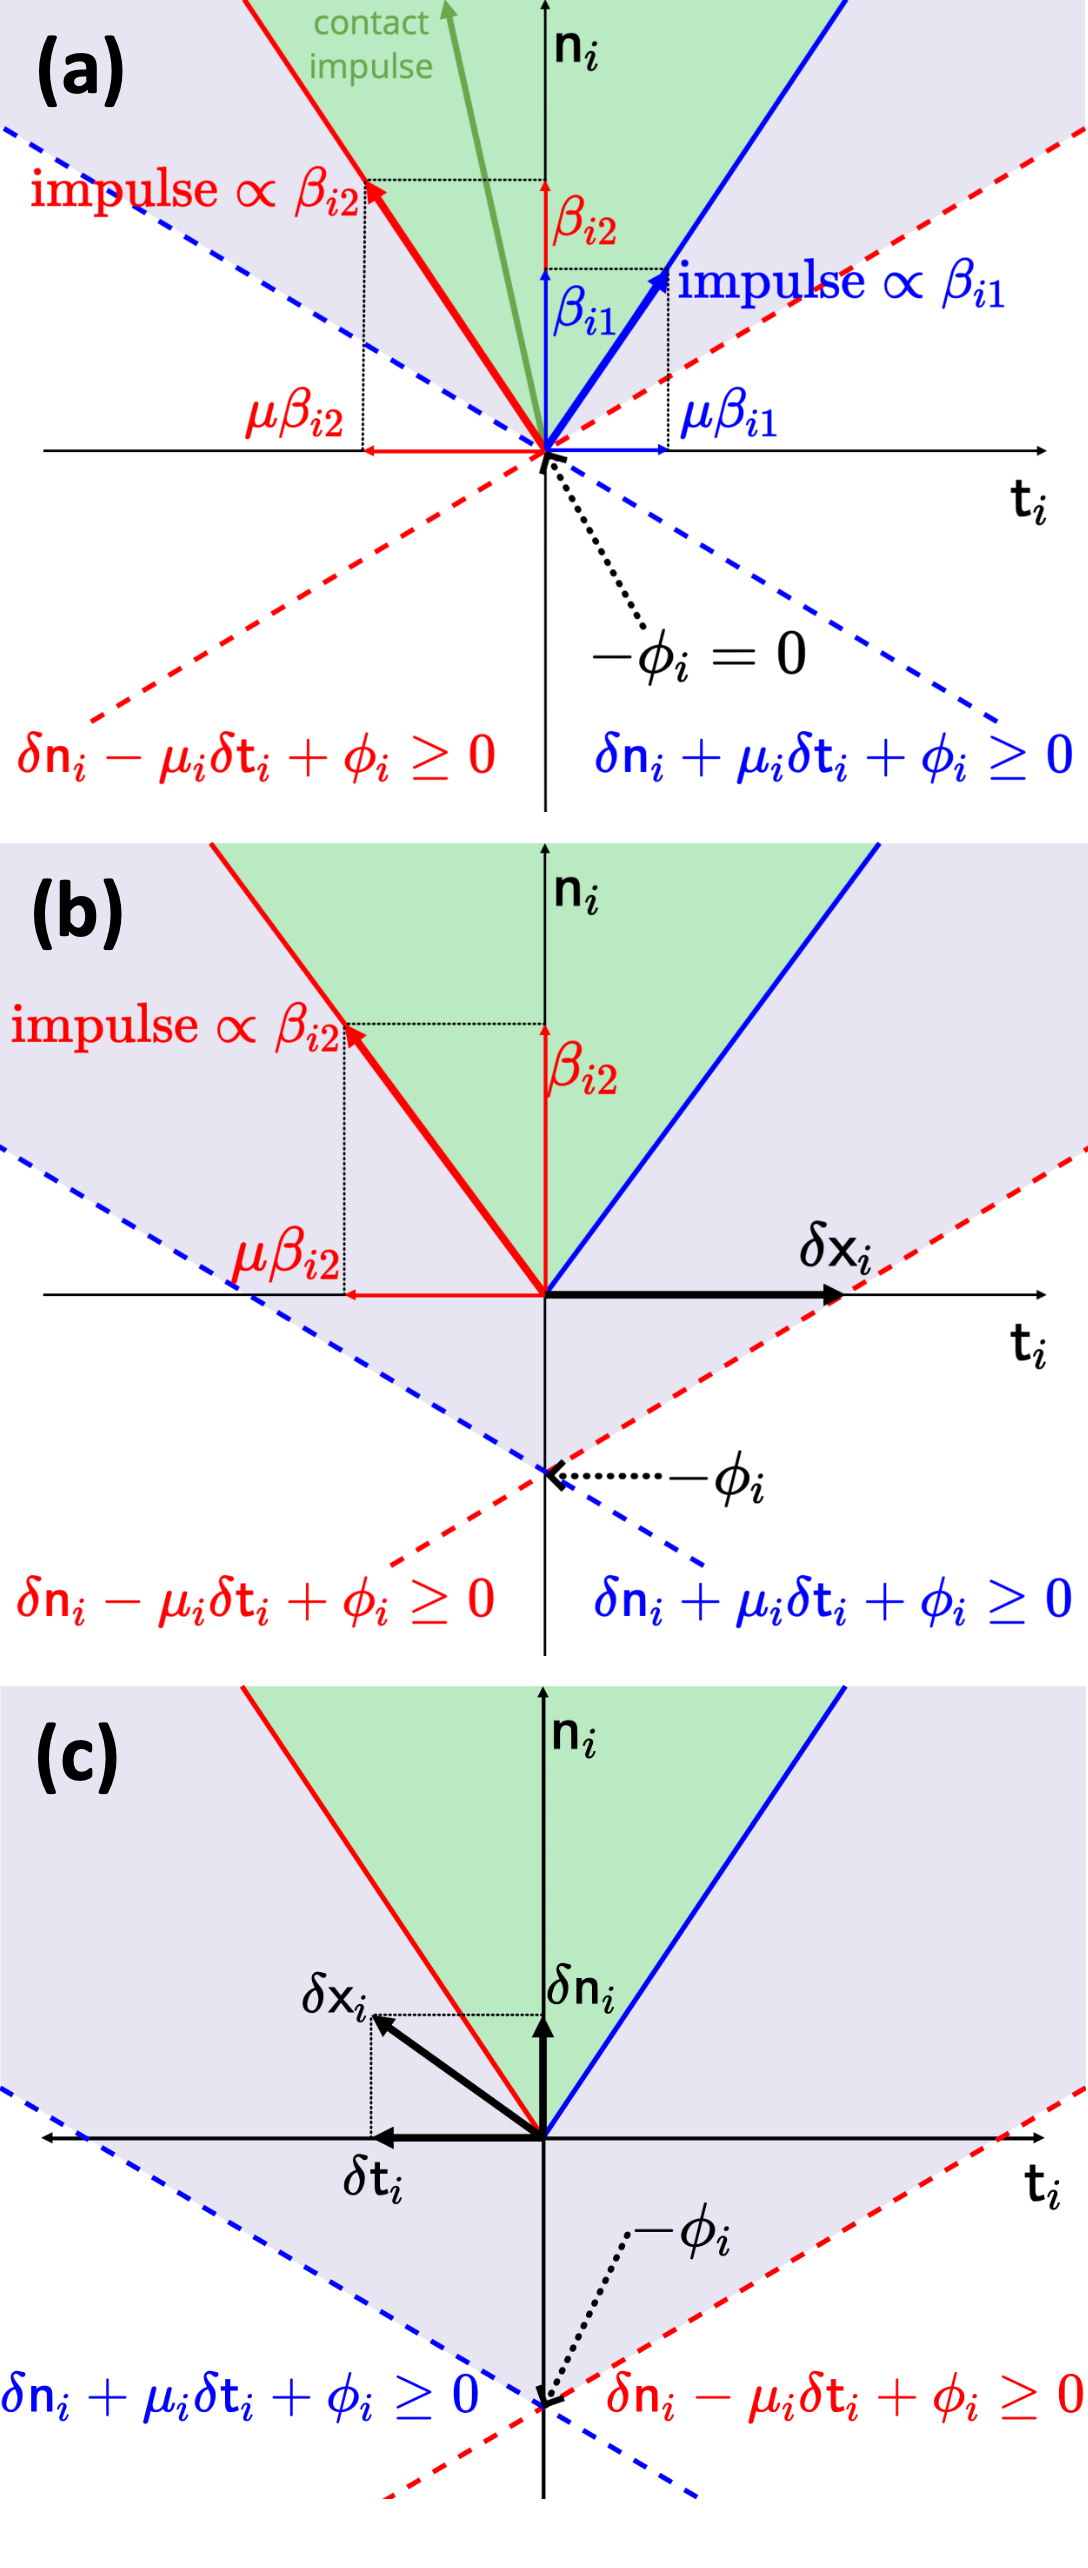
\includegraphics[width=0.53\linewidth]{figures/02_quasi_static_dynamics/anitescu_constraints_detailed.png}
\caption{Anitescu's friction constraints (\ref{eq:anitescu_friction_single_contact_alt}) under different contact modes: (\textbf{a}) sticking, (\textbf{b}) sliding, and (\textbf{c}) separation. The normal and tangent of the contact frame $i$ are denoted respectively by $\mathsf{n}_i$ and $\mathsf{t}_i$. The green shaded area is the friction cone. The purple shaded area is the feasible region of $\delta \mathsf{x}_i$. Constraints corresponding to (\ref{eq:anitescu_friction_single_contact_alt:a}) and (\ref{eq:anitescu_friction_single_contact_alt:b}) are color-coded blue and red, respectively.}
\label{fig:anitescu_constraints_detailed}
\end{figure}

\subsubsection{Sticking (Fig. \ref{fig:anitescu_constraints_detailed}a)} In a sticking contact, $\delta \mathsf{x}_i= 0$, $\phi_i = 0$ and the contact force is inside the friction cone. The conditions for sticking, $\delta \mathsf{x}_i= 0$ and $\phi_i = 0$, imply that $ \delta \mathsf{n}_i + \mu_i \delta \mathsf{t}_i + \phi_i = 0$ and $\delta \mathsf{n}_i - \mu_i \delta \mathsf{t}_i + \phi_i = 0$, i.e. the RHS of (\ref{eq:anitescu_friction_single_contact_alt:a}) and (\ref{eq:anitescu_friction_single_contact_alt:b}) are active. Therefore, both $\beta_{1i}$ and $\beta_{1i}$ can be positive, allowing any contact impulse inside the friction cone. In this case, Anitescu's constraints are identical to Coulomb's friction law. 

\subsubsection{Sliding (Fig. \ref{fig:anitescu_constraints_detailed}b) \label{section:anitescu_friction_sliding}} In a sliding contact, the contact force is on the boundary of the friction cone, and the relative displacement $\delta \mathsf{x}_i$ is horizontal and opposing the friction force. Without loss of generality, we can assume $\beta_{i2}>0$ and $\beta_{i1} = 0$. Hence the RHS of (\ref{eq:anitescu_friction_single_contact_alt:b}) is active, i.e. $\delta \mathsf{x}_i$ is constrained to the red dashed line defined by $ \delta \mathsf{n}_i - \mu_i \delta \mathsf{t}_i + \phi_i = 0$. 
Therefore, $\phi_i = \mu_i \delta \mathsf{t}_i > 0$ per the definition of sliding ($\delta \mathsf{n}_i = 0$ and $\delta \mathsf{t}_i > 0$).
This is the source of the non-physical behavior of Anitescu's friction constraints: when one body is sliding relative to the other, the body slides at a positive distance away from the other body instead of on its surface. In other words, to achieve pure sliding, there must be some separation between the two relative-sliding objects.

\subsubsection{Separation (Fig. \ref{fig:anitescu_constraints_detailed}c)} Separation indicates that there is no contact force, i.e. $\beta_{1i} = \beta_{2i} = 0$. Hence $\delta \mathsf{x}_i$ can take any value in the feasible region defined by the RHS of (\ref{eq:anitescu_friction_single_contact_alt:a}) and (\ref{eq:anitescu_friction_single_contact_alt:b}). For moderate $\mu_i$ and reasonably large $\phi_i$, the feasible region is large enough to accommodate a wide range of velocities.


\subsection{Flaws of Prescribed Robot Motions as Control Input} \label{sec:quasi_static:prescribed_motion_bad}
In Sec. \ref{sec:convex_quasi_dynamic_contact_dynamics}, we model robots as impedance sources, but not all quasi-static models have made this modeling choice. As discussed earlier in Sec. \ref{sec:quasi_static_background}, many existing quasi-static models assume the control input $u$ prescribes robot motions (admittance source) \cite{mason1986mechanics, lynch1996stable, zhou2017fast, hogan2020feedback}, which can be sufficient for planning but insufficient for simulation.
In this subsection, we will illustrate the flaws of modeling robot as prescribed motion for simulation from two complementary perspectives: (\textbf{i}) an example of a parallel-jaw gripper lifting up a sphere, and (\textbf{ii}) bond graphs.

\subsubsection{Parallel-jaw Gripper Lifting Up a Sphere}
The gripper-ball system shown in Fig. \ref{fig:gripper_ball_schematics}a has three actuated DOFs: $x_l$ and $x_r$ are the translation of the left and right gripper fingers along the $x$-axis, respectively; $y$ is the translation of both fingers along the $y$-axis. The two un-actuated DOFs, $x_c$ and $y_c$, are the $x$ and $y$ translation of the sphere.
\begin{figure}
\centering
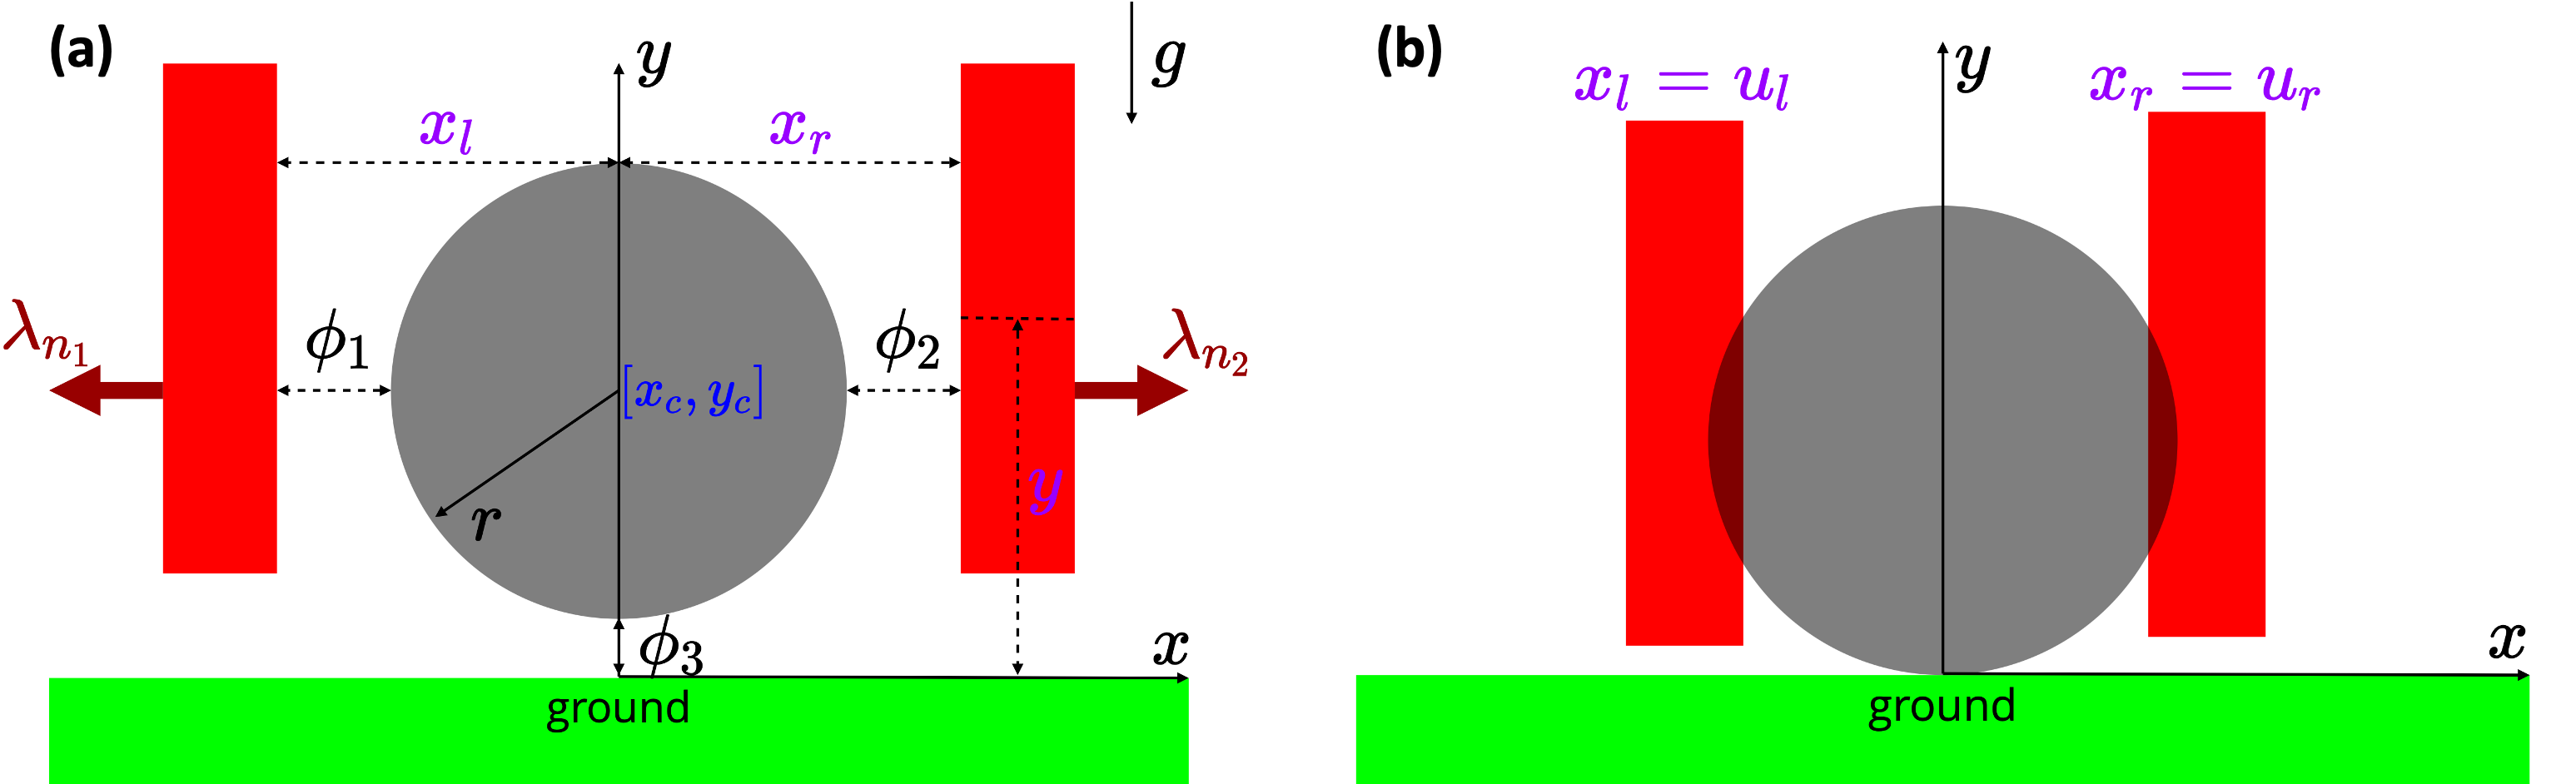
\includegraphics[width=1.0\linewidth]{figures/02_quasi_static_dynamics/gripper_ball_schematics.png}
\caption{(\textbf{a}) A planar quasi-static multibody system. The red rectangles are the actuated gripper fingers, $\qa= [x_l, x_r, y]$ and $u = [u_l, u_r, u_y]$. The gray sphere is the un-actuated manipuland, $\qu = [x_c, y_c]$. $r=0.1\mathrm{m}$. The normal contact forces associated with contact pair 1 and 2 are denoted respectively by $\lambda_{\mathrm{n}_1}$ and $\lambda_{\mathrm{n}_2}$. (\textbf{b}) A grasping command violating the non-penetration constraint.}
\label{fig:gripper_ball_schematics}
\end{figure}

As a consequence of modeling robots as prescribed motions, the robot force balance condition \eqref{eq:q_dynamics_eom:a} is replaced by 
\begin{equation}
\label{eq:naive_quasi_static_robot_motion}
\qa + \delta \qa = u.
\end{equation}

Although seemingly plausible, the simplistic robot dynamics (\ref{eq:naive_quasi_static_robot_motion}) is an ill-posed dynamical system: (\textbf{i}) it is possible to command a $u$ that violates non-penetration constraints; (\textbf{ii}) when two bodies are in contact, the contact force between them can be under-determined \cite{pang2018robust, halm2018quasi}. Instead of belonging to a niche set of contrived corner cases, such issues arise naturally and frequently in even the simplest robotic manipulation tasks. Consider the example in Fig. \ref{fig:gripper_ball_schematics}a, where the fingers are commanded to grasp the sphere. For PD-controlled grippers, it is common to command a small amount of penetration to establish contact forces. However, such commands would penetrate the object, as shown in Fig. \ref{fig:gripper_ball_schematics}b. On the other hand, even if the fingers are commanded to ``graze'' the sphere ($\phi_1 = \phi_2 = 0$), which respects non-penetration constraints, any non-negative contact force $\lambda_{\mathrm{n}_1}$ and $\lambda_{\mathrm{n}_2}$ would satisfy \eqref{eq:q_dynamics_eom:u}. This is problematic if the fingers are also commanded to move up: small contact forces would leave the sphere on the ground, but large contact forces would generate enough friction to lift up the sphere. Modeling control inputs as robot motions simply cannot determine whether the sphere moves with the hand or stays on the table.

Our impedance formulation (\ref{eq:q_dynamics_eom:a}) resolves the ill-posedness of \eqref{eq:naive_quasi_static_robot_motion} by effectively connecting $\qa$ and $u$ using springs with zero rest lengths. To illustrate how the spring helps, we focus on $x_l$, the prismatic joint of left finger in the planar grasping example in Fig. \ref{fig:gripper_ball_schematics}a. Force balance for $x_l$ is given by 
\begin{equation}
\label{eq:force_balance_xl}
    k(u_{l} - x_l) + \lambda_{\mathrm{n}_1} = 0,
\end{equation}
where $k$ is the stiffness of the spring, $k(u_{l} - x_l)$ is the spring force acting on the left finger, and $f_{n_1}$ the force from contact with the sphere.

When the left finger is not in the vicinity of the sphere (Fig. \ref{fig:actuator_with_springs}a), we have $\lambda_{\mathrm{n}_1}=0$, which together with (\ref{eq:force_balance_xl}) implies that $x_l = u_l$. Therefore, in the absence of contact, adding the spring has the same effect as (\ref{eq:naive_quasi_static_robot_motion}). On the other hand, when the left finger is commanded to squeeze the sphere (Fig. \ref{fig:actuator_with_springs}b), $x_l$ and $u_l$ are different due to the non-penetration constraint. The spring force $k(x_l - u_l)$ is balanced by the contact force $\lambda_{\mathrm{n}_1}$. 
\begin{figure}
\centering
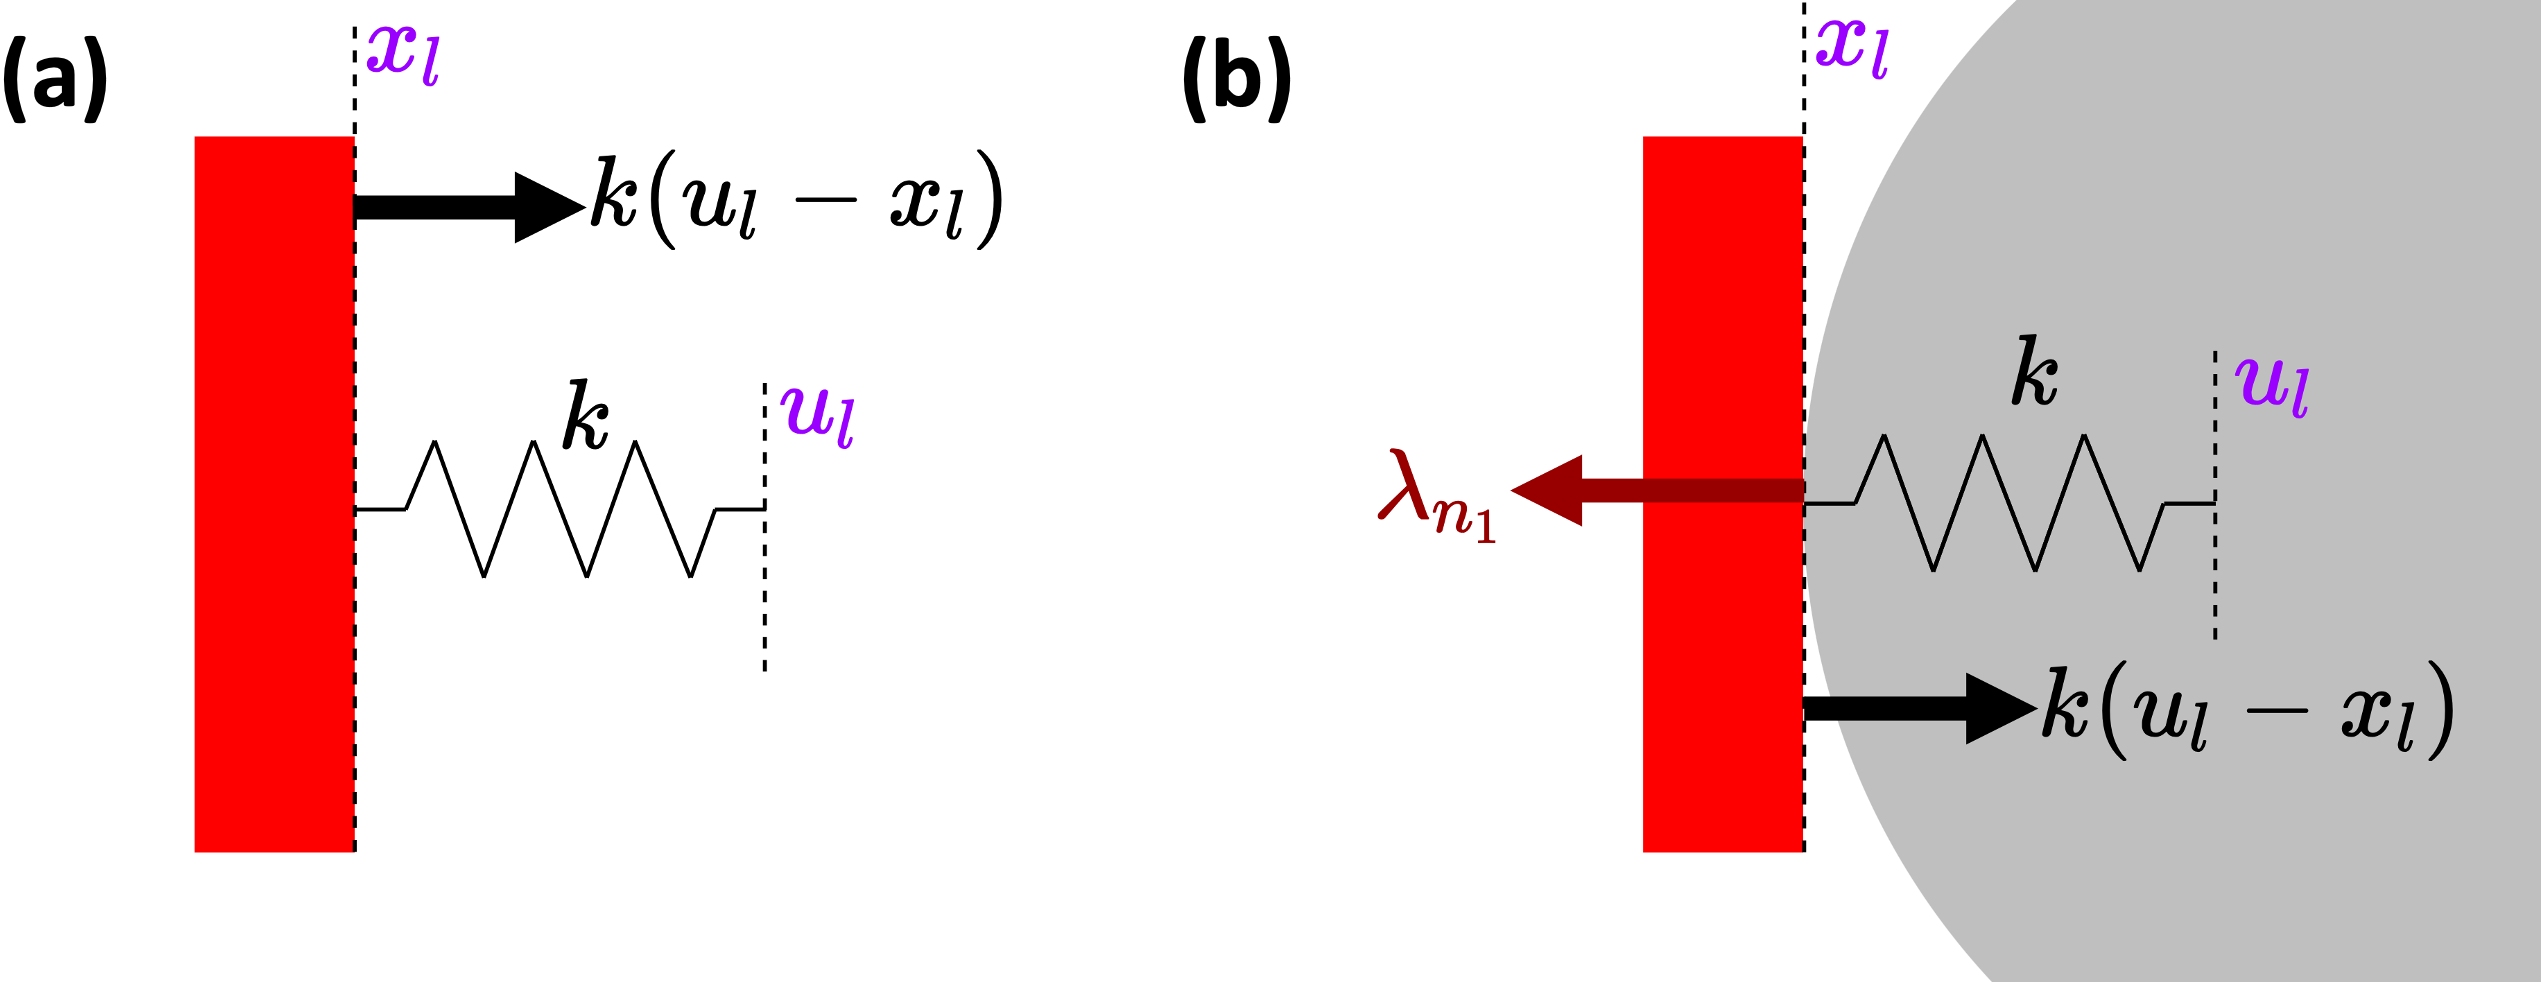
\includegraphics[width=0.90\linewidth]{figures/02_quasi_static_dynamics/actuator_with_springs.png}
\caption{Free-body diagrams of the left finger when it is (\textbf{a}) away from the sphere, and (\textbf{b}) in contact with the sphere.}
\label{fig:actuator_with_springs}
\end{figure}

The addition of the spring resolves both issues with (\ref{eq:naive_quasi_static_robot_motion}): (\textbf{i}) feasibility of the non-penetration constraint is retained by allowing $x_l$ to be different from its commanded value $u_l$; (\textbf{ii}) the magnitude of the contact force is also uniquely determined by the difference between $x_l$ and $u_l$. 

Although adding springs between $\qa$ and $u$ may seem arbitrary, it is equivalent to modeling the actuators as impedances \cite{hogan1985impedance}. For instance, the closed-loop dynamics of the KUKA iiwa arm in joint-impedance mode is:
\begin{equation}
\label{eq:controlled_iiwa_dynamics}
\mathbf{M}(q)\ddot{q} + \left(\mathbf{D}_q + \mathbf{C}(q, \dot{q}) \right) \dot{q}  + \mathbf{K}_q \left(q - u\right) = \tau_{\text{ext}},
\end{equation}
where $q$ is the joint angles of the robot arm, $\mathbf{M}(q)$ the mass matrix, $\mathbf{C}(q, \dot{q})$ the Coriolis force, $\mathbf{K}_q$ the diagonal joint stiffness matrix, $\mathbf{D}_q$ the diagonal damping matrix and $\tau_{\text{ext}}$ the joint torque generated by external contact \cite{ott2008passivity}. Discarding terms related to velocity and acceleration, the second-order dynamics (\ref{eq:controlled_iiwa_dynamics}) becomes
\begin{equation}
    \mathbf{K}_q \left(q - u\right) = \tau_{\text{ext}},
\end{equation}
which can be interpreted as the joint space version of (\ref{eq:force_balance_xl}).

\subsubsection{Bond Graph}
Bond graph is a graphical tool for describing energy flows between components of a dynamical system \cite{bondgraph}. In his seminal work on impedance control, Hogan justified modeling robots as impedances using bond graph analysis \cite{hogan1984impedance}. 

Fig. \ref{fig:bond_graph} shows bond graphs of a 1-DOF quasi-static robot pushing against a wall when the robot is modeled as prescribed motions (admittance) vs. as impedance. Both the robot and the wall are modeled as \emph{flow sources}. In Fig. \ref{fig:bond_graph}a the flows from both sources are constrained to be equal by the \emph{1 junction}, whereas in Fig. \ref{fig:bond_graph}b the flows can be different due to the spring. The flaw of modeling robots as prescribed motions is revealed clearly as a syntax error in the bond graph. In Fig. \ref{fig:bond_graph}a, the 1 junction has two \emph{strong bonds}, both of which dictate the flow. However, the syntax of 1 junction only allows one strong bond per junction.
\begin{figure}
\centering
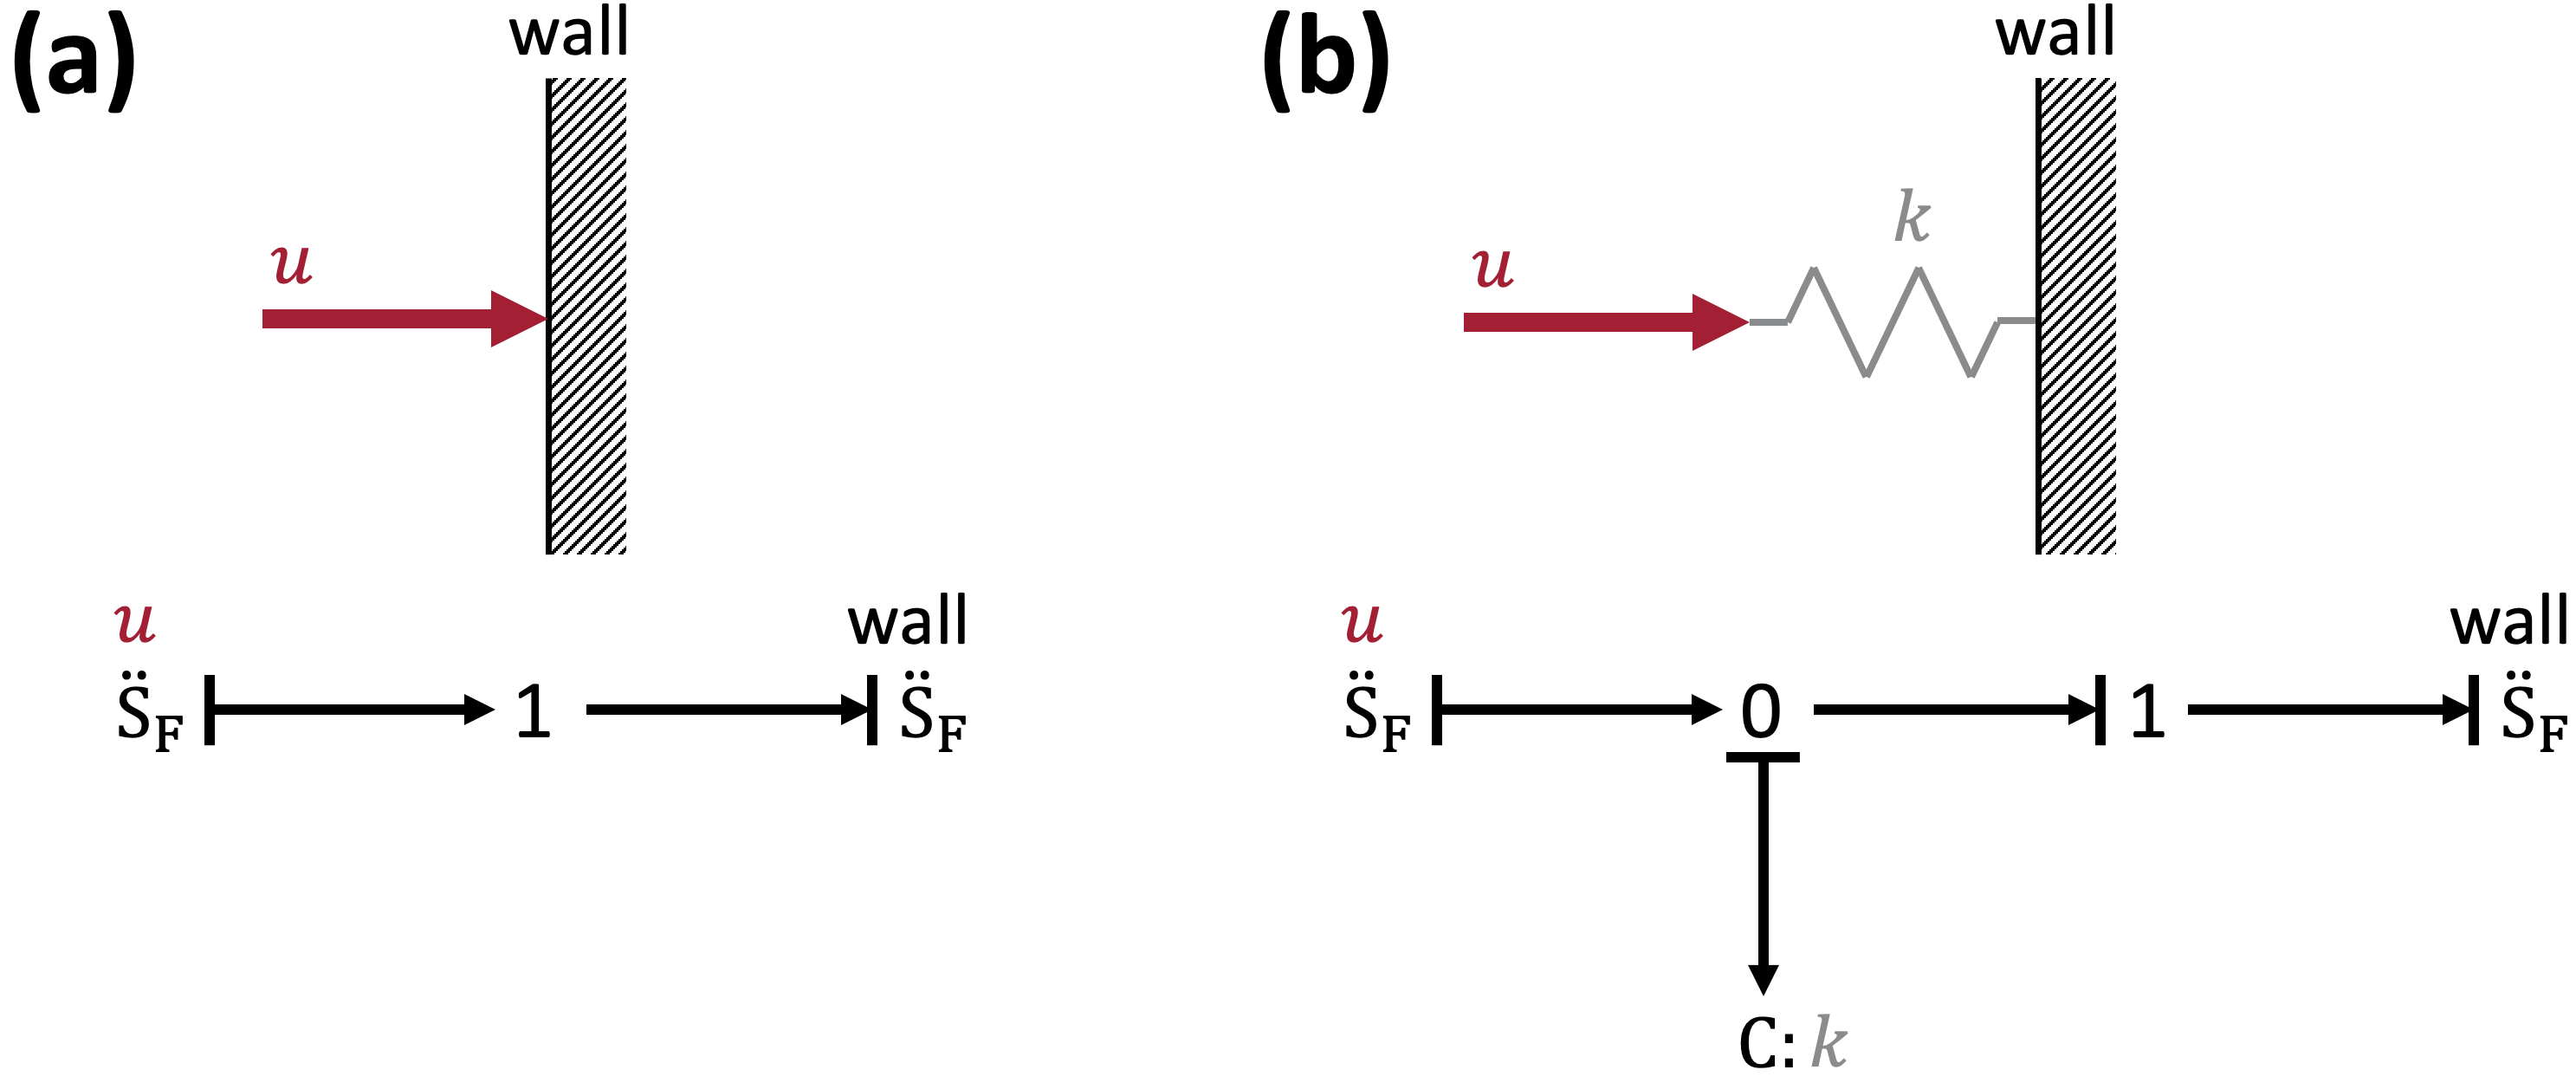
\includegraphics[width=1.0\linewidth]{figures/02_quasi_static_dynamics/bond_graph.png}
\caption{Bond graphs of a 1-DOF robot pushing against the wall. In (\textbf{a}), the robot is modeled as admittance (a prescribed motion). In (\textbf{b}), the robot is modeled as impedance. }
\label{fig:bond_graph}
\end{figure}

\subsection{Experimental Evaluation} \label{sec:quasi_static:experiments}
We want to understand the extent to which simulation accuracy is affected by the ``boundary layer'' due to Anitescu's convex relaxation of the Coulomb friction constraint, which has been illustrated in Sec. \ref{sec:quasi_static:artifacts}. By comparing the proposed CQDC dynamics and a quasi-static LCP formulation on the 2D parallel gripper system using a trajectory that involves multiple contact mode changes, we show that the difference between the two friction formulations is small for typical manipulation tasks.

We also want to ensure that quasi-static simulations stay close to their second-order counterparts for typical manipulation tasks. To this end, we compare the CQDC dynamics against a high-fidelity second-order simulator, Drake's \code{MultibodyPlant} (MBP). To make the comparison as fair as possible, we turn on the semi-analytic primal (SAP) solver \cite{castro2021unconstrained} in MBP. Similar to CQDC, SAP uses Anistecu's convex relaxation of friction constraints \cite{anitescu2006optimization}, and supports implicit integration for PD controllers\footnote{
At the time of writing this thesis, implicit PD controller is still an experimental feature of Drake, pending the merge of \url{https://github.com/RobotLocomotion/drake/pull/17674}.
Implicit integration provides stability at much larger step sizes than explicit integration. The latter has been the default integration scheme in Drake due to the separation of plant and controller into individual systems. In our earlier work \cite{pang2021convex}, we compared CQDC which uses implicit integration against Drake's MBP, which is an unfair comparison due to the difference in integration schemes. 
}.
Our comparison shows that both CQDC and SAP are stable at large integration step sizes (at least $0.5\mathrm{s}$), but CQDC seems to be better at respecting non-penetration constraints as the step size gets larger, possibly because CQDC enforces non-penetration constraints directly on positions rather than on velocities.


\subsubsection{2D Parallel Gripper}
We study the ``boundary layer'' effect of the CQDC dynamics by comparing it against an LCP-based quasi-static formulation \cite{pang2021convex} which enforces the same object and robot equations of motion in \eqref{eq:q_dynamics_eom}, but models friction using linear complementarity constraints \cite{stewart1996implicit} instead of the cone complementarity constraints \eqref{eq:friction_constraints}. 

The comparison is done on the 2D grasping example introduced in Fig. \ref{fig:gripper_ball_schematics} using a gripper trajectory that induces multiple contact mode changes between the fingers and the sphere. As the system is planar, CQDC's SOCP formulation \eqref{eq:q_dynamic_socp} reduces to the QP formulation \eqref{eq:q_dynamics_planar_qp}. We use the QP formulation for the comparison in this example. 

The simulation time step $h$ is set to $0.01\mathrm{s}$; the weight of the sphere is $10\mathrm{N}$; the stiffness for all actuated DOFs is $1000 \mathrm{N / m}$ and a friction coefficient of $0.5$ is used for all contacts. The regularization constant $\epsilon$ in \eqref{eq:q_dynamics_eom:u} is set to 0. We will use $c_{\mathrm{n}_i} \coloneqq \lambda_{\mathrm{n}_i} / h$ and $c_{\mathrm{f}_i} \coloneqq \lambda_{\mathrm{t}_i} / h$ to denote the normal and tangent components of the contact forces.

\begin{figure}
\centering
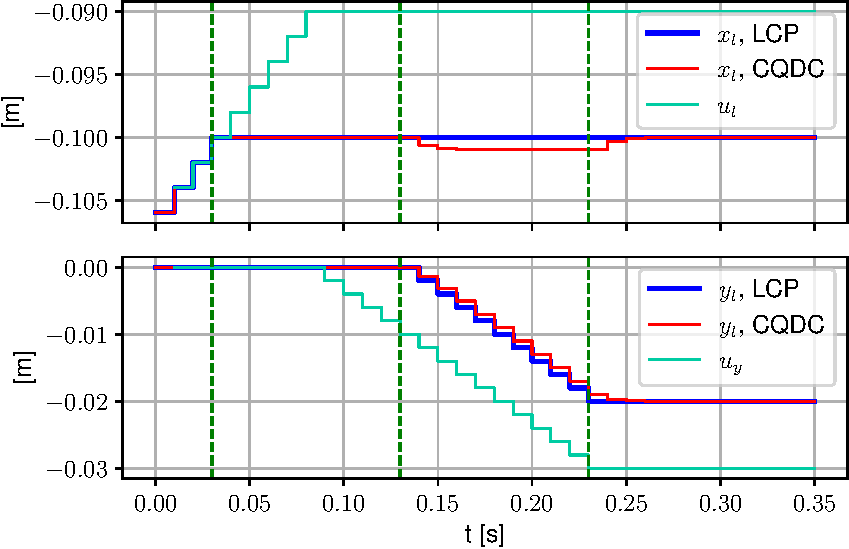
\includegraphics[width=0.75\linewidth]{figures/02_quasi_static_dynamics/xy_cmd_vs_xy_true.pdf}
\caption{Commanded and actual left finger positions for the system defined in Fig. \ref{fig:gripper_ball_schematics}, as simulated by LCP and the proposed CQDC dynamics (\ref{eq:q_dynamics_planar_qp}). 
Recall that $x_l$ and $u_l$ are respectively the commanded and actual $x$-coordinate of the left finger; $y_l$ and $u_y$ are respectively the commanded and actual $y$-coordinate of both fingers.
The right finger is not shown, as the motions and forces of the left and right fingers are symmetric about the $y$-axis. 
The green dashed vertical lines indicate contact mode changes: separation to sticking at $t=0.03\mathrm{s}$; sticking to sliding at $t=0.13\mathrm{s}$; sliding to sticking at $t=0.23\mathrm{s}$.}
\label{fig:xy_cmd_vs_xy_true}
\end{figure}

As shown in Fig. \ref{fig:xy_cmd_vs_xy_true}, the grippers start $0.006\mathrm{m}$ away from the surface of the sphere. They are first commanded to translate horizontally, touching the sphere at $t = 0.03\mathrm{s}$. The grippers continue to squeeze the object until $t = 0.08 \mathrm{s}$. Accordingly, $c_{\mathrm{n}_1}$ grows from $0\mathrm{N}$ to $10\mathrm{N}$, while $\phi_1$ stays at 0. As shown in Fig. \ref{fig:contact_force_distance}, this behavior is reproduced by both the LCP formulation and the CQDC dynamics \eqref{eq:q_dynamics_planar_qp}.

The grippers are then commanded to pull the ball downward into the ground. Although initially resisted by friction, the downward commands eventually overcome friction and slipping between the ball and the fingers starts at $t = 0.13 \mathrm{s}$. In the LCP simulation, $c_{\mathrm{n}_1}$, $c_{\mathrm{f}_1}$ and $\phi_1$ remain constant despite the contact mode transition from sticking to sliding. In the CQDC simulation, however, as sliding starts at $t = 0.13 \mathrm{s}$, a small increase in $\phi_1$ is observed, which, as explained in Section. \ref{section:anitescu_friction_sliding}, is needed by sliding under Anitescu's friction constraints. In both the LCP and CQDC simulations, $c_{\mathrm{n}_3}$ grows with the friction $c_{\mathrm{f}_1}$ in order to keep the sphere in force balance.

The downward commands stop at $t = 0.24 \mathrm{s}$, and the contact mode switches back to sticking from sliding. Once again, $c_{\mathrm{n}_1}$, $c_{\mathrm{f}_1}$ and $\phi_1$ remain constant in the LCP formulation. In contrast, the ``boundary layer'' created by sliding in the CQDC dynamics disappears as sliding stops.

\begin{figure}
\centering
\subfloat[Simulated by quasi-static LCP.]{
	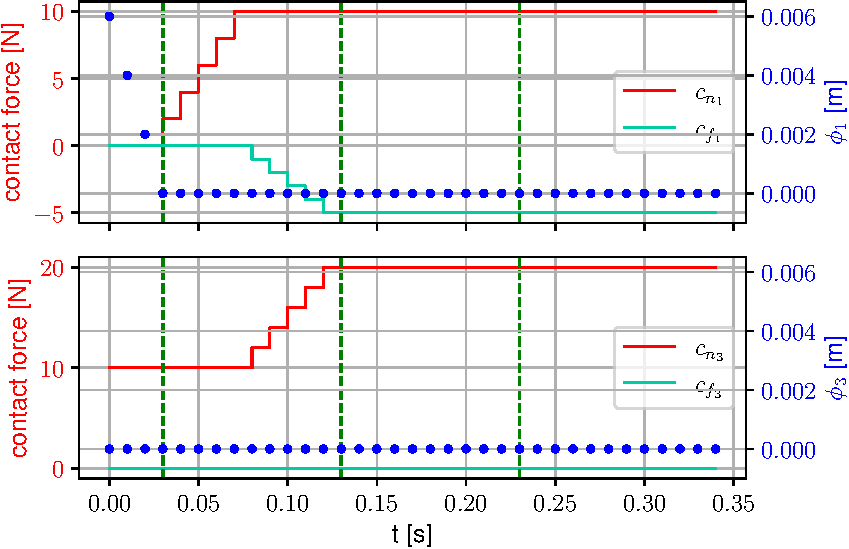
\includegraphics[width=0.75\linewidth]{figures/02_quasi_static_dynamics/contact_force_distance_lcp.pdf}
	\label{fig:contact_force_distance_lcp}
}\\
\subfloat[Simulated by the proposed CQDC dynamics (\ref{eq:q_dynamics_planar_qp}).]{
	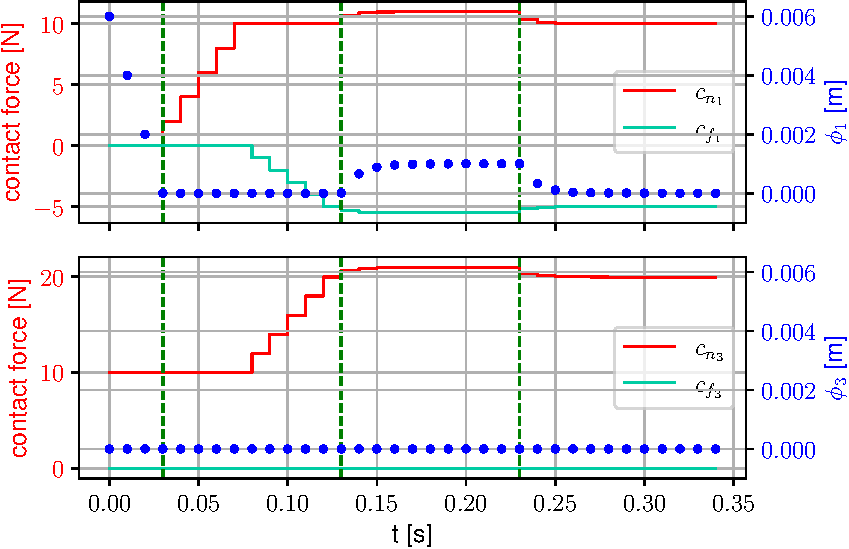
\includegraphics[width=0.75\linewidth]{figures/02_quasi_static_dynamics/contact_force_distance_qp.pdf}
	\label{fig:contact_force_distance_qp}
}
\caption{Contact force and signed distance at contact 1 and 3 of the gripper-sphere system defined in Fig. \ref{fig:gripper_ball_schematics}.}
\label{fig:contact_force_distance}
\end{figure}

\subsubsection{Iiwa Trajectory Tracking}
Our first comparison between CQDC and SAP involves tracking a reference joint-angle trajectory $q_\mathrm{ref}(\cdot)$ on a gravity-compensated and PD-controlled iiwa arm. The task only involves the smooth closed-loop dynamics of the arm \eqref{eq:controlled_iiwa_dynamics}, and does not involve any external contact. The starting and ending configurations of the reference trajectory are shown in Fig. \ref{fig:iiwa_trajectory_tracking}a and Fig. \ref{fig:iiwa_trajectory_tracking}b, respectively. We interpolate between the two configurations using a cubic spline, with maximum velocity in the middle and zero velocity at the two ends. We will denote the trajectory simulated by the CQDC dynamics as $q_\mathrm{CQDC}(\cdot)$, and SAP by $q_\mathrm{SAP}(\cdot)$.

\begin{figure}[h]
\centering
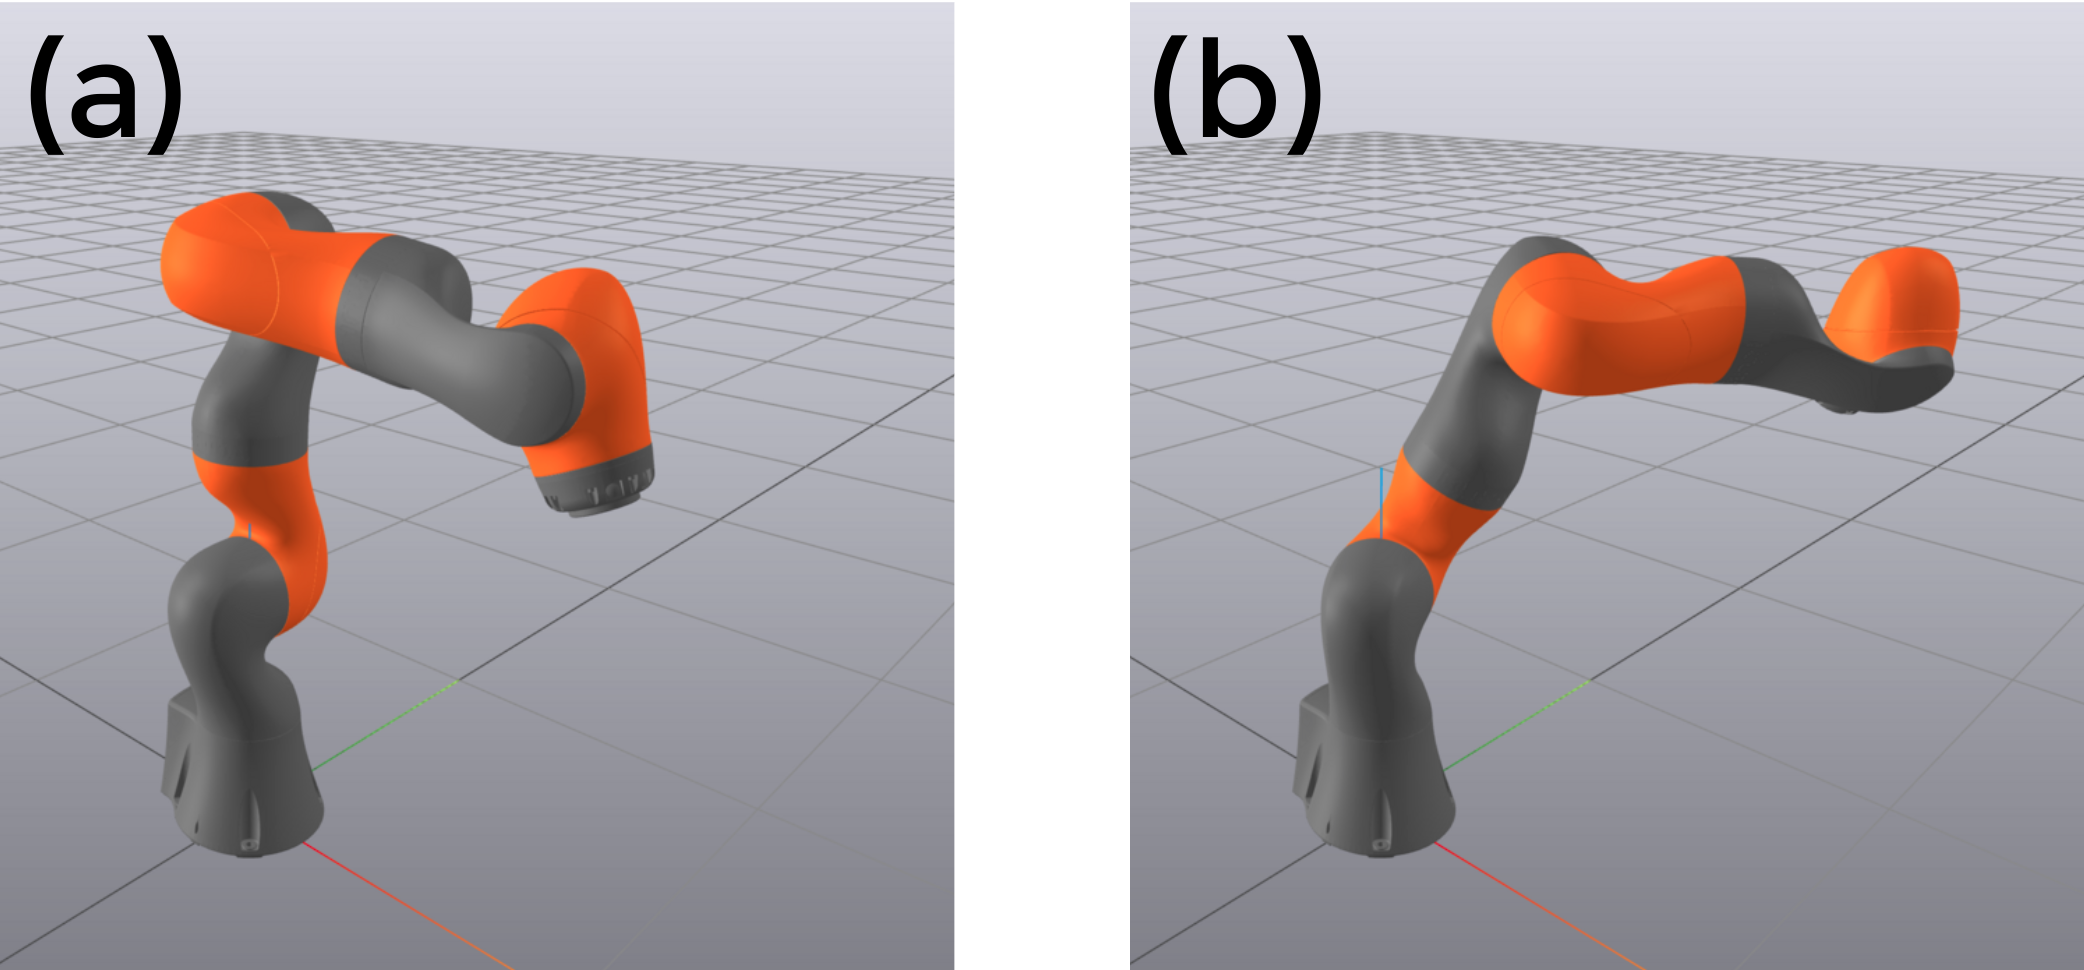
\includegraphics[width=0.70\linewidth]{figures/02_quasi_static_dynamics/iiwa_trajectory_tracking.png}
\caption{Starting (\textbf{a}) and ending (\textbf{b}) configurations of the reference joint-angle trajectory $q_\mathrm{ref}(\cdot)$.}
\label{fig:iiwa_trajectory_tracking}
\end{figure}

To evaluate the performance of the two simulators, we first define the mean error $\Delta(\cdot,\cdot)$ between two joint-angle trajectories $q_\mathrm{1}(\cdot)$ and $q_\mathrm{2}(\cdot)$ as
\begin{equation}
\label{eq:mean_trajectory_error}
\Delta(q_\mathrm{1}, q_\mathrm{2}) \coloneqq 
\frac{1}{T}
\int^T_{0} d(q_\mathrm{1}(t), q_\mathrm{2}(t))\mathrm{d}t,
\end{equation}
where $T$ denotes the duration of the trajectories; $d(\cdot, \cdot)$ is the distance metric for the space of joint angles, which is simply the Euclidean 2-norm.

For different simulation step sizes $h$, the mean errors between simulated and reference trajectories, i.e. $\Delta(q_\mathrm{CQDC/SAP}, q_\mathrm{ref})$, are shown in Fig. \ref{fig:iiwa_trajectory_tracking_error_vs_time_step}. The error increases with $h$, but remains small even for very large $h$ ($h=0.5\mathrm{s}$). In addition, as CQDC has no inertia, it tends to be slightly better at tracking the reference, especially as $h$ gets smaller.

\begin{figure}[h]
\centering
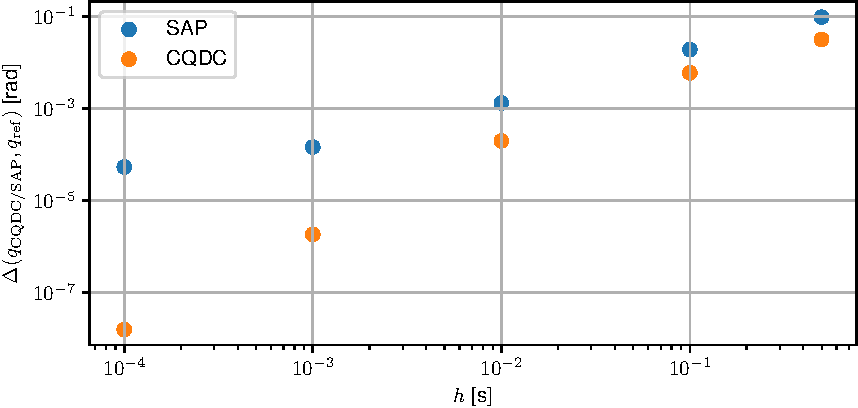
\includegraphics[width=0.8\linewidth]{figures/02_quasi_static_dynamics/iiwa_trajectory_tracking_error_vs_time_step.pdf}
\caption{Mean tracking error $\Delta(q_\mathrm{CQDC/SAP}, q_\mathrm{ref})$ for trajectories simulated using the CQDC dynamics or SAP at different simulation step sizes $h$.}
\label{fig:iiwa_trajectory_tracking_error_vs_time_step}
\end{figure}


\subsubsection{Box Stacking with Iiwa}
Our second comparison between CQDC and SAP focuses on a complex 3D system with many contacts, as shown in Fig. \ref{fig:iiwa_cube_stacking}. The system has 10 cubes and 69 DOFs. The task is the robot picking up the red-and-grey cube and placing it on the stack. There is on average 56 contacts per time step during the execution of the task.
\begin{figure}
\centering
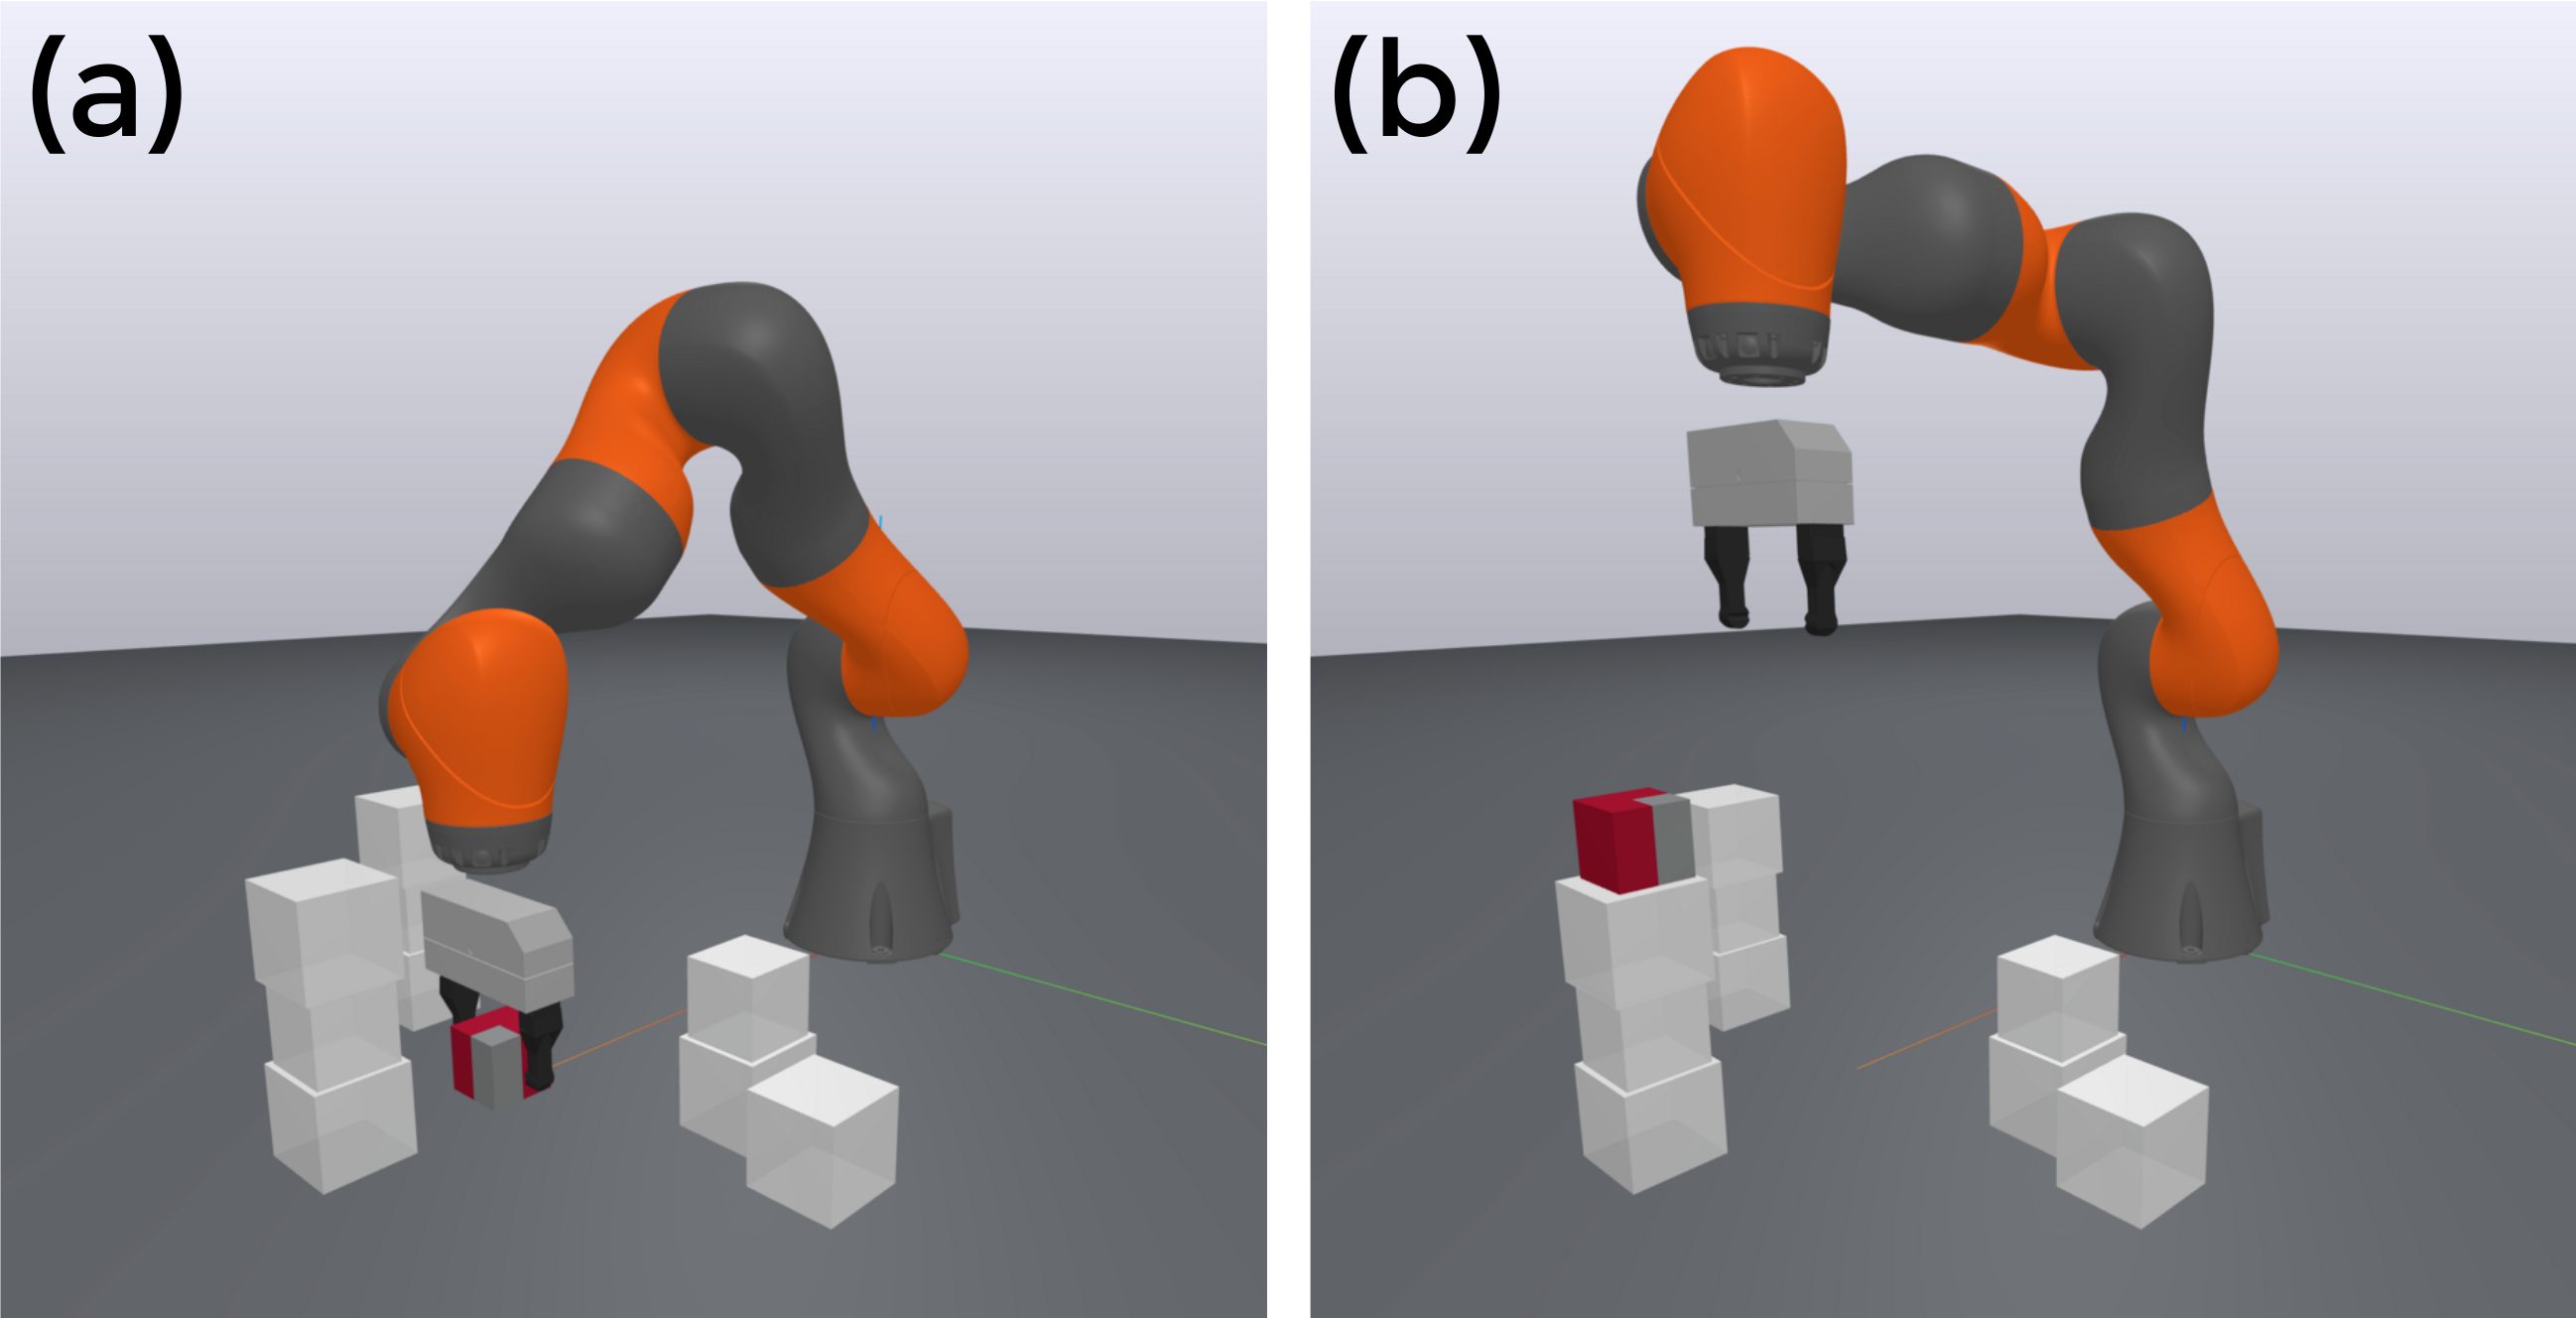
\includegraphics[width=0.75\linewidth]{figures/02_quasi_static_dynamics/start_and_final_configurations.png}
\caption{KUKA IIWA robot stacking cubes. The red-and-grey cube has a quadrant colored grey to indicate its orientation. The red-and-grey cube starts off on the ground (\textbf{a}) and is placed on a stack of cubes and rotated by 90 degrees (\textbf{b}).}
\label{fig:iiwa_cube_stacking}
\end{figure}

Firstly, although both CQDC and SAP are stable for large step sizes (at least $h=0.5\mathrm{s}$), CQDC is accurate for all step sizes, whereas the accuracy of SAP starts to degrade significantly as $h$ crosses a threshold. 
Similar to the iiwa trajectory tracking example, we compare trajectories of the red-and-grey cube using the mean error defined by \eqref{eq:mean_trajectory_error}. Instead of comparing against a reference trajectory, we define the \emph{ground truth} trajectory of the box, $q_\mathrm{GT}^\mathrm{u}(\cdot)$, as the trajectory generated by SAP using $h=5 \times 10^{-5} \mathrm{s}$.
As shown in Fig. \ref{fig:error_vs_time_step}, the mean error of the box pose between CQDC and the ground truth, $\Delta (q_\mathrm{CQDC}^\mathrm{u}, q_\mathrm{GT}^\mathrm{u})$, remains small up to $h=0.1\mathrm{s}$ and is still moderate at $h=0.5\mathrm{s}$, indicating that a large $h$ can be used for planning without impacting accuracy.
In contrast, $\Delta (q_\mathrm{SAP}^\mathrm{u}, q_\mathrm{GT}^\mathrm{u})$ becomes large for $h \geq 0.01 \mathrm{s}$.
\begin{figure}
\centering
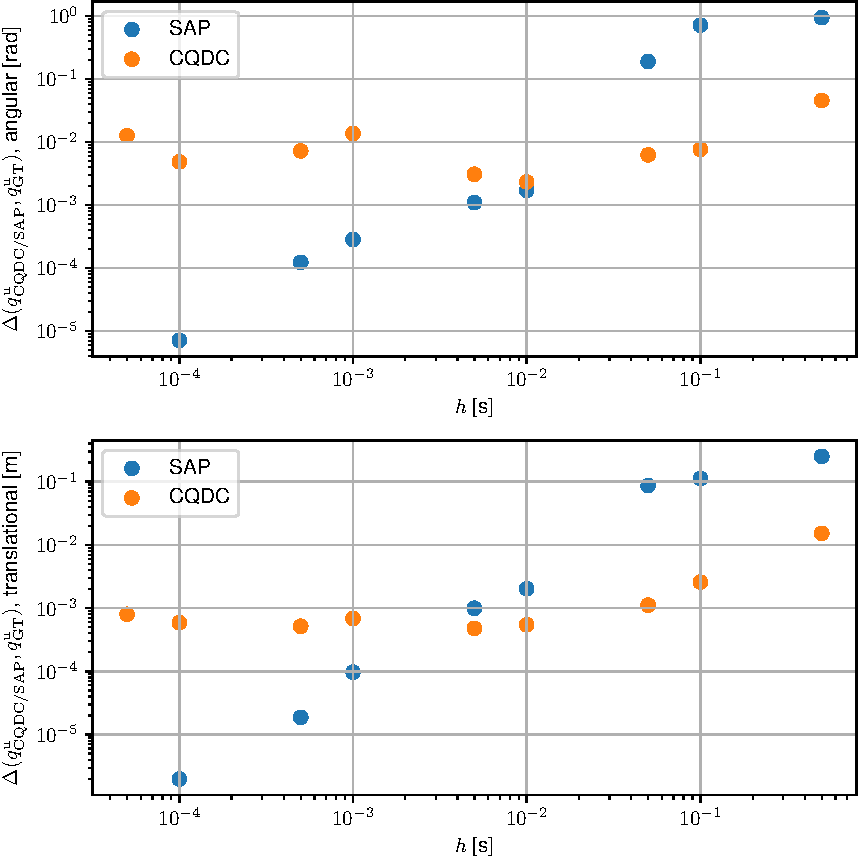
\includegraphics[width=0.8\linewidth]{figures/02_quasi_static_dynamics/error_vs_time_step.pdf}
\caption{Angular and translational mean error of the pose of the red-and-grey box, $\Delta (q_\mathrm{CQDC/SAP}^\mathrm{u}, q_\mathrm{GT}^\mathrm{u})$, at different step sizes $h$.
As shown in Fig. \ref{fig:iiwa_cube_stacking}, the box is picked up, rotated, and placed on the stack of cubes.
The ground truth trajectory, $q_\mathrm{GT}^\mathrm{u}$, is defined as the trajectory generated by SAP with $h=5\times10^{-5}\mathrm{s}$.
In the computation of the mean error $\Delta(\cdot, \cdot)$, the distance function $d(\cdot, \cdot)$ is the Euclidean 2-norm for translation, and the absolute difference in angle for rotation.
}
\label{fig:error_vs_time_step}
\end{figure}

The reason behind the larger error of SAP at larger step sizes is shown in Fig. \ref{fig:iiwa_cube_stacking_sap_vs_cqdc}. With SAP, it appears that contacts become softer as $h$ increases, eventually leading to boxes sinking into each other and the ground. 
\begin{figure}
\centering
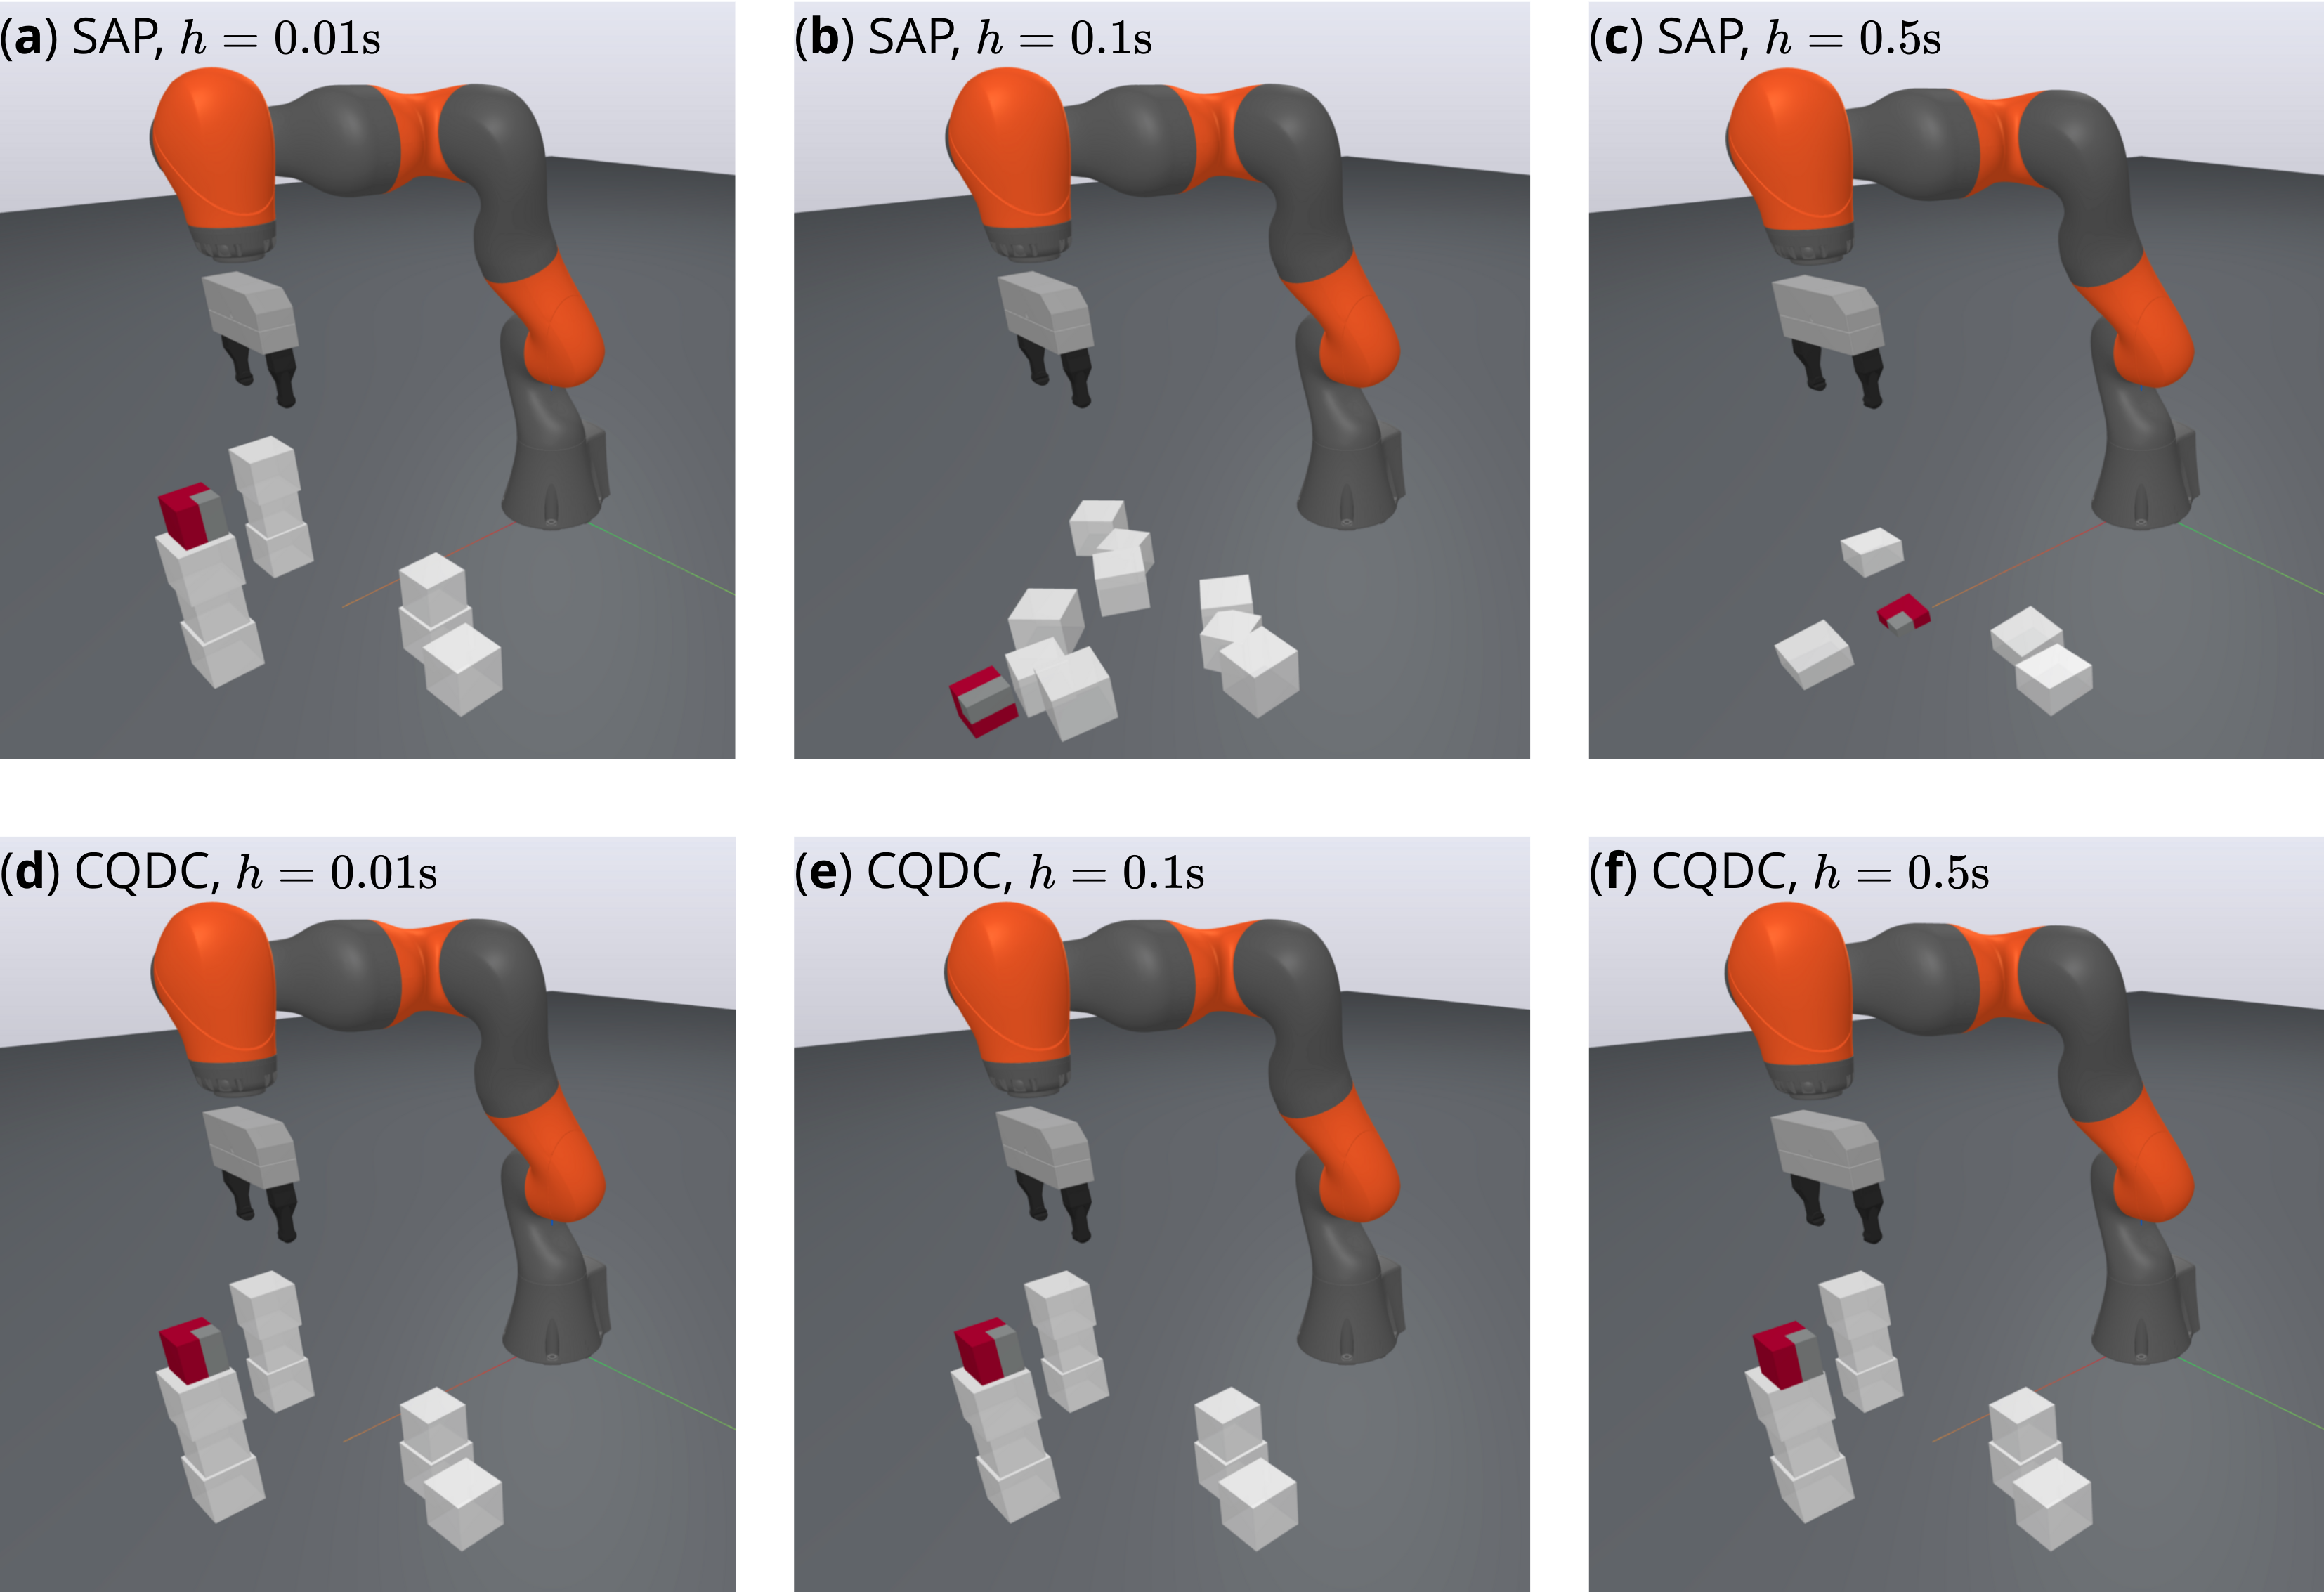
\includegraphics[width=1.0\linewidth]{figures/02_quasi_static_dynamics/sap_vs_cqdc.png}
\caption{Final configurations of the box stacking task shown in Fig. \ref{fig:iiwa_cube_stacking}, simulated using SAP (\textbf{a}-\textbf{c}) and CQDC (\textbf{d}-\textbf{f}).}
\label{fig:iiwa_cube_stacking_sap_vs_cqdc}
\vspace{-0.5cm}
\end{figure}

Good simulation accuracy by the CQDC dynamics at large $h$ is also evident in the pose trajectory of the box, which is shown in Fig. \ref{fig:cube_pose}. The translational trajectories are almost identical to the ground truth for all $h$ except $h=0.5\mathrm{s}$, but even at $h=0.5\mathrm{s}$ the error is just slightly more than 1cm. There is also no significant deviation of the object orientation from the ground truth. 
\begin{figure}
\centering
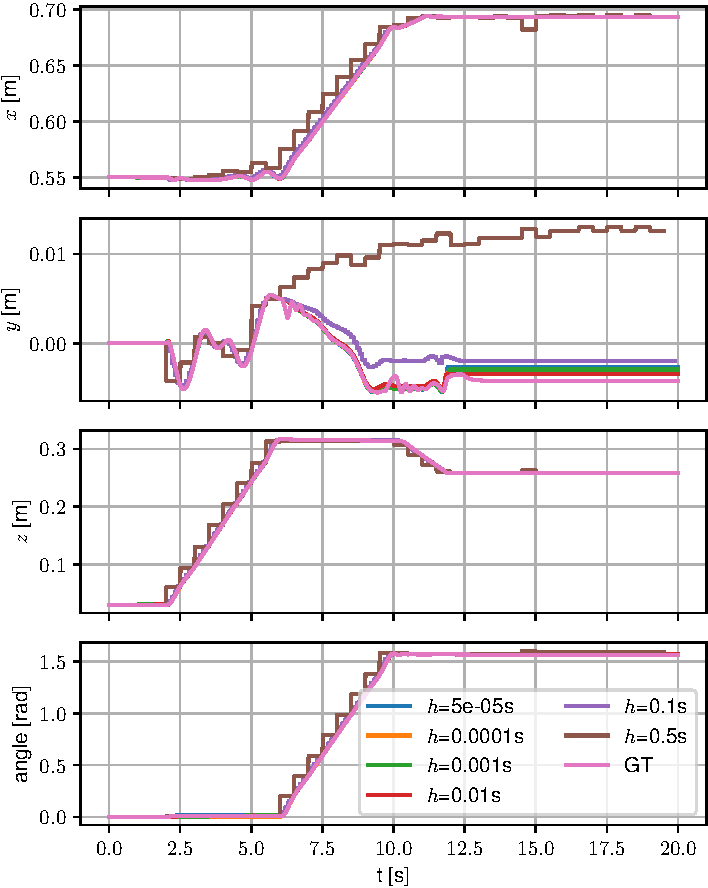
\includegraphics[width=0.9\linewidth]{figures/02_quasi_static_dynamics/box0_pose.pdf}
\caption{Trajectories of the red cube in Fig. \ref{fig:iiwa_cube_stacking}, including the ground truth (GT) and the ones generated using the CQDC dynamics with different step sizes $h$. $x$, $y$ and $z$ are the cube's center of mass coordinates in world frame. Angle comes from the axis-angle representation of the cube's orientation relative to world frame. Here the angle plot represents a rotation about the world $y$-axis by 90 degrees. The larger $y$ error at $h=0.5\mathrm{s}$ is caused by the gripper clipping the corner of the red-and-grey box when the gripper retreats from the box after placing it on the top of the stack. Due to the large $h$, the gripper's motion is interpolated between an upward segment and a horizontal segment. This error is visible by the difference of a few pixels between Fig. \ref{fig:iiwa_cube_stacking_sap_vs_cqdc}e
and Fig. \ref{fig:iiwa_cube_stacking_sap_vs_cqdc}f.
}
\label{fig:cube_pose}
\end{figure}

Lastly, the CQDC dynamics (\ref{eq:q_dynamic_socp}) scales well with the number of DOFs and contacts. The mean time of solving SOCP (\ref{eq:q_dynamic_socp}) using Gurobi \cite{gurobi} for the box stacking task in Fig. \ref{fig:iiwa_cube_stacking} is less than 10ms on a Mac mini with Intel i7-8700B CPU and 64GB of RAM. 

\newpage
\section{Smoothing of Contact Dynamics} \label{sec:smoothing}
This section discusses how the proposed CQDC dynamics (Sec. \ref{sec:q_dynamics:cqdc}) can be smoothed, so that we can efficiently make good local linear approximations that are useful for planning.
We will begin with a summary of the randomized and analytic smoothing schemes proposed in \cite[Section II]{pang2022global} (Sec. \ref{sec:smoothdynamics}). 
We will then discuss how the proposed quasi-static dynamics model readily supports both randomized (Sec. \ref{sec:randomizedmoothing}) and analytic smoothing (Sec. \ref{sec:analyticsmoothing}), and how the two schemes are related (Sec. \ref{sec:smoothing_equivalence}). 


\subsection{Smoothing Schemes for Dynamical Systems}
\label{sec:smoothdynamics}
This subsection summarizes three different smoothing schemes for dynamical systems of the form $x_+ = f(x, u)$ \eqref{eq:f_x_u}. The smoothing schemes are (\textbf{i}) analytic smoothing, (\textbf{ii}) first-order randomized smoothing and (\textbf{iii}) zeroth-order randomized smoothing.

Although the three schemes all compute the same quantity, they require different levels of access of the dynamics $f(\cdot, \cdot)$. Analytic smoothing utilizes the structure of $f(\cdot, \cdot)$ to efficiently compute a smoothed version of it, and therefore requires white-box access to $f(\cdot, \cdot)$. In contrast, randomized smoothing schemes achieve smoothing via sampling: first-order randomized smoothing needs black-box access to $f(\cdot, \cdot)$, $\DfDx{f}{x}(\cdot, \cdot)$ and $\DfDx{f}{u}(\cdot, \cdot)$, whereas zeroth-order randomized smoothing only needs black-box access to $f(\cdot, \cdot)$.

We use $(\mathbf{A}(\bar{x},\bar{u}),\mathbf{B}(\bar{x},\bar{u}),c(\bar{x},\bar{u}))$ to parameterize the linear system $\bar{f}$ that best describes $f$ around some nominal point $(\bar{x},\bar{u})$, 
\begin{equation}
    \begin{aligned}
    \bar{f}(x,u) = \mathbf{A}(\bar{x},\bar{u})\underbrace{(x-\bar{x})}_{=:\delta x } + \mathbf{B}(\bar{x},\bar{u})\underbrace{(u-\bar{u})}_{=:\delta u} + c(\bar{x},\bar{u}).
    \end{aligned}
\end{equation}
For dynamical systems, the Taylor expansion requires the system Jacobian, 
\begin{equation}\label{eq:linearization}
    \begin{aligned}
    \mathbf{A}(\bar{x},\bar{u}) & = \frac{\partial}{\partial x}f(x,u)|_{x=\bar{x},u=\bar{u}} \\
    \mathbf{B}(\bar{x},\bar{u}) & =\frac{\partial}{\partial u}f(x,u)|_{x=\bar{x},u=\bar{u}} \\
    c(\bar{x},\bar{u}) & = f(\bar{x},\bar{u}).
    \end{aligned}
\end{equation}
The \emph{smooth surrogate} of $f(x,u)$ can be defined as
\begin{equation}
\label{eq:smooth_surrogate_definition}
    f_\rho(x,u) \coloneqq \mathbb{E}_{w\sim\rho}[f(x+w^x,u+w^u)],
\end{equation}
where $\rho$ is a probability distribution, $w^x$ is the component of $w$ that corresponds to $x$, and $w^u$ is defined similarly. The model parameters of the locally linear model $\bar{f}_\rho$ are given as follows:
\begin{equation}
\label{eq:ABc_rho}
    \begin{aligned}
    \mathbf{A}_\rho(\bar{x},\bar{u}) & =  \frac{\partial}{\partial x}\mathbb{E}_{w\sim\rho}[f(x+w^x,u+w^u)]|_{x=\bar{x},u=\bar{u}} \\
    \mathbf{B}_\rho(\bar{x},\bar{u}) & =  \frac{\partial}{\partial u}\mathbb{E}_{w\sim\rho}[f(x+w^x,u+w^u)]|_{x=\bar{x},u=\bar{u}} \\
    c_\rho(\bar{x},\bar{u}) & = \mathbb{E}_{w\sim\rho}[f(\bar{x}+w^x,\bar{u}+w^u)].
    \end{aligned}
\end{equation}
In the remaining sections, we shorthand the notation and refer to the model parameters as a matrix instead of a function for compactness (e.g. $\mathbf{A}_\rho$ instead of $\mathbf{A}_\rho(\bar{x},\bar{u})$). 

\subsubsection{Analytic Smoothing}
Analytic smoothing is done by explicit computation of $f_\rho$ as defined in \eqref{eq:smooth_surrogate_definition}. In general, it is difficult to compute $f_\rho$ for arbitrary functions $f$ and smoothing kernels $\rho$. In Sec. \ref{sec:analyticsmoothing}, we introduce a method for computing $f_\rho$ when $f$ is the CQDC dynamics.

\subsubsection{First-Order Randomized Smoothing}
We use the following estimators for first-order randomized smoothing of dynamical systems,
\begin{subequations}
\label{eq:montecarlo_ABc}
\begin{align}
\mathbf{A}_\rho & \approx \textstyle \frac{1}{N}\sum^N_{i=1} \left[\textstyle\frac{\partial}{\partial x}f(\bar{x}+w_i^x,\bar{u}+w_i^u\right] \quad w_i\sim \rho \label{eq:montecarlo_ABc:A} \\ 
\mathbf{B}_\rho & \approx \textstyle \frac{1}{N}\sum^N_{i=1} \left[\textstyle\frac{\partial}{\partial u}f(\bar{x}+w_i^x,\bar{u}+w_i^u)]\right] \quad w_i\sim \rho \\ 
c_\rho & \approx \textstyle \frac{1}{N}\sum^N_{i=1} \left[\textstyle f(\bar{x}+w_i^x,\bar{u}+w_i^u)]\right] \quad w_i\sim \rho \label{eq:montecarlo_ABc:c} 
\end{align}
\end{subequations}
where $\partial f/\partial x$, and $\partial f/\partial u$ are Jacobians of the dynamics.

\subsubsection{Zeroth-Order Randomized Smoothing}
We estimate the gradients using least-squares when $\rho$ is Gaussian:
\begin{equation}
\label{eq:montecarlo_ABc_zero}
\mathbf{A}_\rho,\mathbf{B}_\rho  = \underset{\mathbf{A,B}} {\text{argmin}}\textstyle\sum^N_{i=1}
 \| f(\bar{x}+w_i^x,\bar{u}+w_i^u) - \mathbf{A} w_i^x - \mathbf{B} w_i^u - c_\rho\|^2_2
\end{equation}
where $c_\rho$ is computed with \eqref{eq:montecarlo_ABc:c}.


\subsection{Randomized Smoothing of Contact Dynamics} \label{sec:randomizedmoothing}
We follow the method in Sec. \ref{sec:smoothdynamics} in order to perform randomized smoothing of the contact dynamics. For first-order randomized smoothing, we utilize \eqref{eq:montecarlo_ABc} with access to gradients of the contact dynamics obtained in Sec.\ref{sec:quasi_dynamic_derivatives}. We similarly do zero-order randomized smoothing using \eqref{eq:montecarlo_ABc_zero}. As the state consists of only the system configuration $q$ for quasi-static systems, we assume we compute a local model around some nominal state-input pair $(\bar{q},\bar{u})$ from here onward.

However, there is a caveat in the randomized smoothing scheme: if the sampling distribution $\rho$ has infinite support, the sampled state $\bar{q} + w^q_i$ could violate the non-penetration constraint for rigid-bodies, i.e. $\phi(\bar{q} + w^q_i) < 0$ for some $i$.

Although reasoning about the dynamics $f(q, u)$ with an infeasible (penetrating) $q$ may seem ill-posed \cite{contactkalmanfilter}, we can \emph{define} the dynamics from an infeasible $q$ as the projection of $q$ to the ``nearest'' point in the feasible (non-penetrating) set. The notion of nearest can be defined in terms of the work required to move the system configuration by $\dq$, which is precisely the quadratic cost \eqref{eq:q_dynamic_socp:cost} (divided by the step size $h$). This projection problem can then be written as
\begin{subequations}
\label{eq:projection_as_optimization}
\begin{align}
\underset{\dq}{\minimize} \; &\frac{1}{2} \dq^\intercal \mathbf{Q} \dq + b^\intercal \dq, \; \text{subject to} \\
& \phi_i(q + \delta q) \geq 0, \; i \in \{1 \dots \nC\}, \label{eq:projection_as_optimization:constraint}
\end{align}
\end{subequations}
where \eqref{eq:projection_as_optimization:constraint} is the non-linear non-penetration constraint. 

While the projection in \eqref{eq:projection_as_optimization} is difficult to solve in general, we can linearize the constraint \eqref{eq:projection_as_optimization:constraint} in order to locally approximate the problem as a QP. When the constraint is linearized, the problem remarkably becomes equivalent to the frictionless special case of the CQDC dynamics \eqref{eq:q_dynamic_socp}. In other words, projection is simply another interpretation of what the CQDC dynamics does within the penetrating regime, and no other explicit treatment is required for projection other than the evaluation of CQDC dynamics. In practice, due to the local nature of linearization, we use a low-variance distribution $\rho$ to sample states, though higher variance can be used for inputs.

When samples within the penetrating regime are projected onto the boundary of the feasible set and then averaged, the expected value of such a distribution creates a \emph{stochastic force field} that pushes the object away from feasible set's boundary. We illustrate this phenomenon through a simple example. 

\begin{example}\label{ex:projection}\normalfont\textbf{(The Stochastic Force Field)} Consider the dynamics of an unactuated 1D block with a wall occupying $q \leq 0$ (Fig. \ref{fig:projection}a), such that the physical dynamics is identity \emph{if} the block is in a non-penetrating configuration, $f(q)=q$ if $q\geq 0$. The dynamics within the penetrating regime is not well-defined physically; yet, applying the quasi-dynamic equations of motions \eqref{eq:projection_as_optimization} to this system gives 
\begin{subequations}
\label{eq:projection}
\begin{align}
\underset{\delta q}{\minimize} \; &\frac{1}{2} m (\delta q)^2, \; \text{subject to} \\
& q + \delta q \geq 0.
\end{align}
\end{subequations}
which has the following solution,
\begin{equation}
\label{eq:1d_projection_solution}
f(q) = q + \delta q =  \begin{cases}
    q & \text{ if } q \geq 0  \text{ (no penetration) }\\
    0 & \text{ else } \text{ (penetration) }\\
\end{cases}
\end{equation}

One interpretation of \eqref{eq:1d_projection_solution} is that configurations inside the wall gets projected onto the wall. By taking an average according to such dynamics, the expectation pushes the box away from the wall as illustrated in Fig. \ref{fig:projection}, which creates a \emph{stochastic force field}. Note that with this interpretation, the gradients are also well-defined within the penetrating regime - an infinitesimal change of position in the penetrating configuration does not have any effect on the location of projection in this example, thus $\partial f(q)/\partial q=0$ if $q < 0$. For more complex geometries, the location of projection changes due to changes in the surface, which we connect back to the presence of the $\partial \mathbf{J}/\partial q$ and $\partial \phi/\partial q$ terms in \eqref{eq:DdqDq}.

\begin{figure}
\centering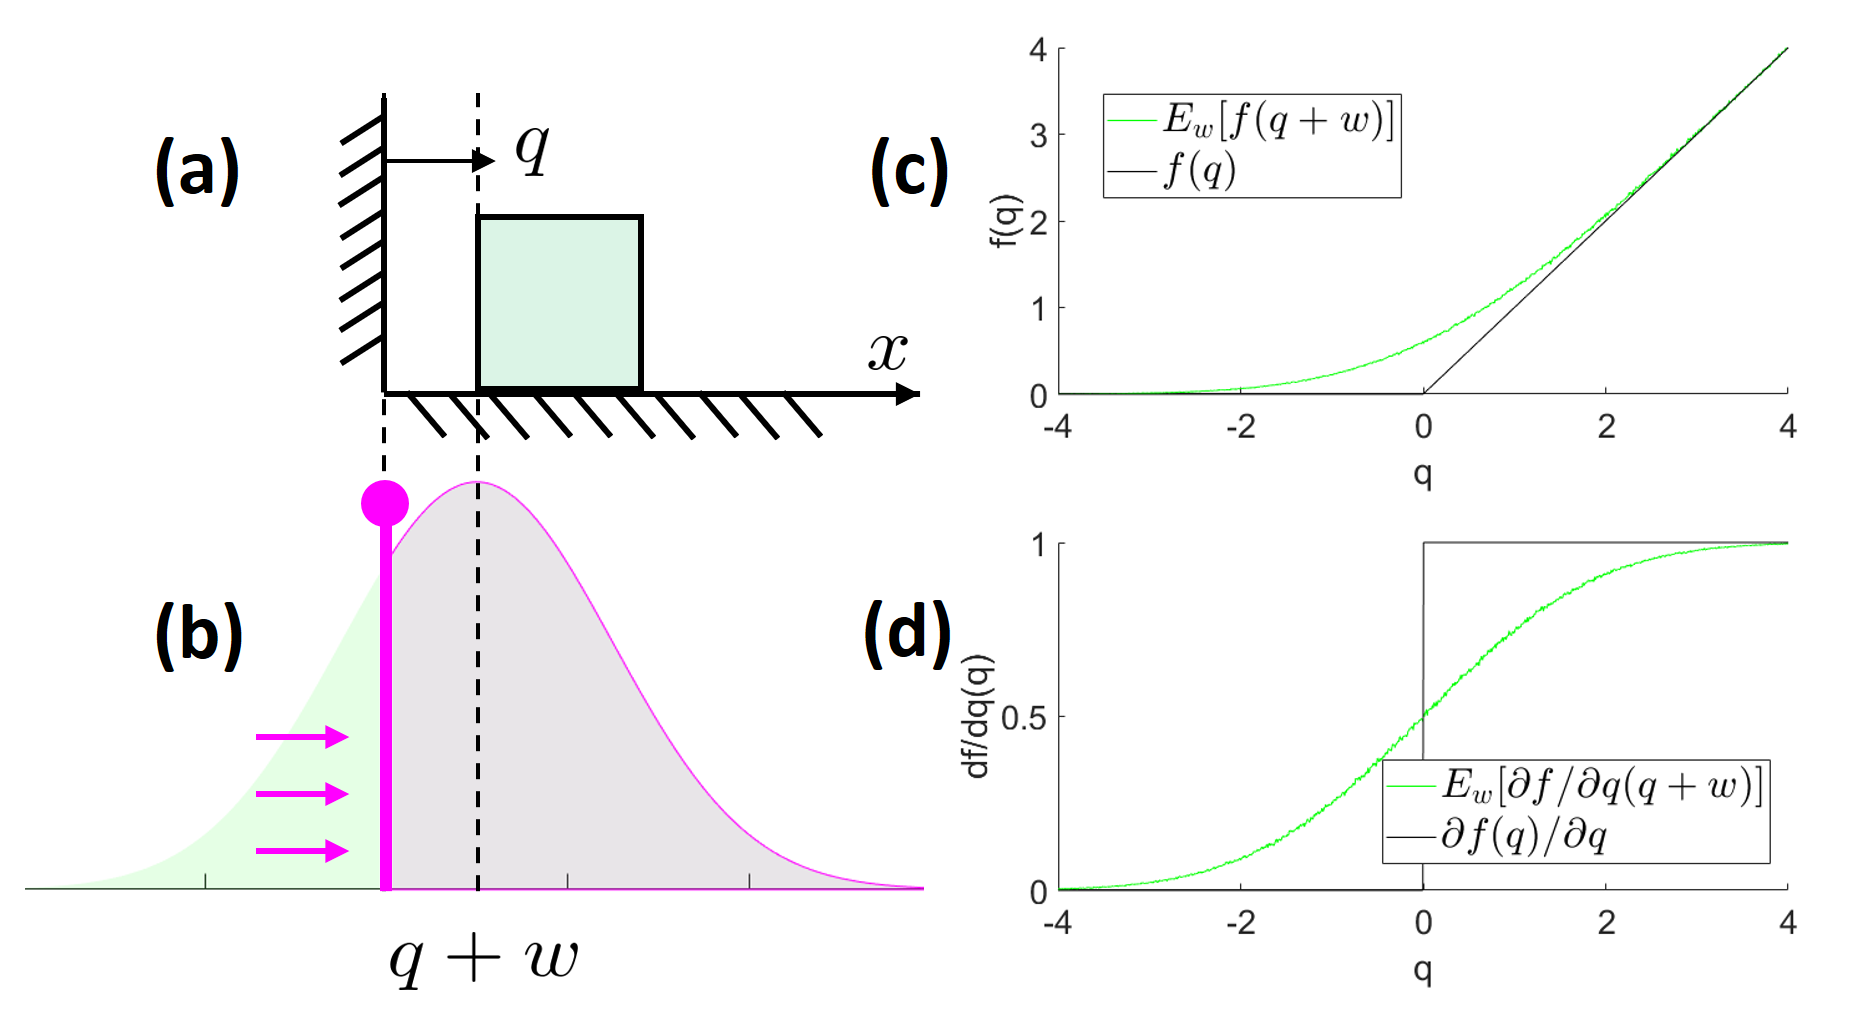
\includegraphics[width = 0.90\textwidth]{figures/02_quasi_static_dynamics/projection.png}
\caption{Figure for Example \ref{ex:projection}, where quasi-dynamics of motion is interpreted as a projection operator. (\textbf{a}) Illustration of the system. (\textbf{b}) Distribution of $q + w$ (green) and $f(q + w)$ (pink). Note that the samples for which $q+w_i<0$ have been projected onto the surface into a delta function, and the expectation of the pink distribution lies on the right side of $q$, creating a stochastic force field effect. (\textbf{c}) CQDC dynamics and its randomized smoothed version. (\textbf{d}) Gradients of the CQDC dynamics obtained with first-order randomized smoothing.}
\label{fig:projection}
\end{figure}
\end{example}

\subsection{A Smoothed Contact Dynamics Model}\label{sec:analyticsmoothing}
Both randomized smoothing schemes only involve repeatedly solving the CQDC dynamics \eqref{eq:q_dynamic_socp} and/or its gradient \eqref{eq:q_dynamics_AB}. In contrast, analytic smoothing (Sec.\ref{sec:smoothdynamics}) of the CQDC dynamics \eqref{eq:q_dynamic_socp} is not as straightforward, since the solution to an optimization problem does not give easy access to explicit forms from which we can analytically design smooth surrogates.

To perform analytic smoothing,  we can convert the hard constraints in a convex program into costs using a penalty method. Specifically, we convert the constrained program \eqref{eq:q_dynamic_socp} into an unconstrained convex program using the log-barrier function, a common technique in the interior-point method for convex conic programs, with weight $\kappa$:
\begin{equation}
\label{eq:q_dynamics_log}
\underset{\dq}{\minimize} \; \frac{1}{2} \dq^\intercal \mathbf{Q} \dq + b^\intercal \dq - \frac{1}{\kappa} \sum_{i=1}^{\nC} \log \left[\frac{(\Jn[i] \dq + \phi_i)^2}{\mu_i^2} - (\Jt[i]\dq)^\intercal \Jt[i]\dq \right],
\end{equation}
whose solution converges to the solution of \eqref{eq:q_dynamic_socp} as $\kappa \rightarrow \infty$ \cite[\textsection 11.3 and \textsection 11.6]{boyd2004convex}.

From a contact mechanics perspective, the log-barrier formulation is motivated by relaxing the strict complementary slackness condition of the CQDC dynamics to allow contact forces at a distance. In fact, the optimality conditions of \eqref{eq:q_dynamics_log} are almost identical to the KKT conditions of \eqref{eq:q_dynamic_socp}. The only difference is that complementary slackness \eqref{eq:friction_constraints:complementary_slackness} is relaxed from $v_i^\intercal \lambda_i = 0$ to $v_i^\intercal \lambda_i = \kappa^{-1}$ by the log barrier formulation ($v_i$ is defined in \eqref{eq:friction_constraints:v_i}).

The log-barrier term in \eqref{eq:q_dynamics_log} can be interpreted as the potential of a force field whose strength is inversely proportional to the distance to the boundary of the constraint \cite[p.567]{boyd2004convex}. For moderate values of $\kappa$, constraints can exert forces even though they are not active, achieving a smoothing effect similar to the ``force-at-a-distance'' relaxation of complementarity constraints, which are commonly used in planning through contact methods such as \cite{posa2014direct, howell2022dojo}. We will further illustrate this similarity in Example \ref{ex:equivalence}.

From $\dq^\star$, the solution to the smoothed dynamics \eqref{eq:q_dynamics_log}, we can directly compute the smoothed gradient $\A_\rho$ and $\B_\rho$ in the same way as \eqref{eq:q_dynamics_AB}. Once again, the derivatives of $\dq^\star$ with respect to $q$ and $u$ are computed by applying the implicit function theorem to the optimality condition of \eqref{eq:q_dynamics_log}, which only consists of the stationarity condition due to the absence of conic constraints.

To solve \eqref{eq:q_dynamics_log}, we implemented an in-house solver using Newton's method \cite[\textsection 9.5]{boyd2004convex}, and find that our out-of-the-textbook implementation works robustly and reliably for all numerical experiments in Sec. \ref{sec:traj_opt} and \ref{sec:rrt_results}.


\subsection{The Smooth Contact Model as ``Analytic Smoothing''} \label{sec:smoothing_equivalence}
In Sec. \ref{sec:smoothdynamics}, we saw that randomized and analytic smoothing can be interpreted as different methods of computing an equivalent quantity. Here, we show with examples that (\textbf{i}) for simple systems, we can derive the sampling distribution $\rho$ needed to obtain the smoothing given by the log-barrier-based analytic smoothing scheme; (\textbf{ii}) for more complex systems, randomized smoothing schemes using a Gaussian $\rho$ and the log-barrier-based analytic smoothing scheme result in qualitatively-similar smoothed dynamics.

\begin{example}\label{ex:equivalence} \normalfont(\textbf{Equivalence of Smoothing Schemes})
We start with the 1D frictionless system in Fig. \ref{fig:equivalence}a, whose dynamics is an instance of the frictionless CQDC dynamics \eqref{eq:q_dynamic_socp}:
\begin{equation}
\label{eq:q_dynamics_1d_cart}
\begin{aligned}
\underset{\dqa}{\minimize} \; &\frac{1}{2} hk_a (\dqa)^2 - h \ka (u - \qa) \dqa, \; \text{subject to} \\
&\qa + \dqa \geq 0,
\end{aligned}
\end{equation}

The KKT conditions of \eqref{eq:q_dynamics_1d_cart} are also the equations of motion of the system:
\begin{subequations}
\label{eq:wallcartdynamics}
\begin{align} 
h k_\mathrm{a} \left(\qa + \dqa - u\right) &= \lambda, \\
0 \leq \left(\qa + \dqa  \right) &\perp \lambda \geq 0,
\end{align}
\end{subequations}
which has the explicit solution
\begin{equation}
    q^\mathrm{a}_+ = \qa + \dqa =  \begin{cases}
        u & \text{ if } u \geq 0  \text{ (no contact) }\\
        0 & \text{ else } \text{ (contact) }\\
    \end{cases}.
\end{equation}

Also as an instance of \eqref{eq:q_dynamics_log}, \eqref{eq:q_dynamics_1d_cart} can be smoothed analytically by converting the constraint into a cost using the log-barrier function:
\begin{equation}
\underset{\dqa}{\minimize} \; \frac{1}{2} hk_a (\dqa)^2 - h \ka (u - \qa) \dqa - \frac{1}{\kappa} \log \left(\qa + \dqa \right),    
\end{equation}
whose optimality condition is obtained by setting the gradient of the smoothed cost to 0, yielding the equations of motion of the smoothed system: 
\begin{equation}
\label{eq:smooth_1d_cart}
hk_\mathrm{a}(\qa + \dqa - u) = \frac{1}{\kappa}\bigg(\frac{1}{\qa + \dqa}\bigg).
\end{equation}

The right-hand side of \eqref{eq:smooth_1d_cart} can be interpreted as an impulse whose magnitude is inversely proportional to the distance to the wall. Calling this impulse $\beta$, we note that
\begin{equation}
\label{eq:complementarity_simple}
    \beta (\qa + \dqa) = \kappa^{-1},
\end{equation}
which is analogous to the common bilinear relaxation to the complementarity constraint for contact \cite{posa2014direct, howell2022dojo}\footnote{
In trajectory optimization, the complementarity constraint is usually relaxed to $\beta (\qa + \dqa) \leq \kappa^{-1}$, instead of the equality in \eqref{eq:complementarity_simple}. The inequality gives the constraint non-empty interior, making it numerically better.
}.

The solution to \eqref{eq:smooth_1d_cart} is given by 
\begin{equation}
    q^\mathrm{a}_+=\frac{1}{2}\left(u + \sqrt{u^2 + \frac{4}{\kappa h^2k^2_\mathrm{a}}}\right)
\end{equation}
which is equivalent to randomized smoothing of the original dynamics under the following elliptical distribution
\begin{equation}
    \rho(w) = \sqrt{\frac{4\sigma }{(w^\intercal\sigma w + 4)^3}},
\end{equation}
where $\sigma\coloneqq hk\kappa $.
\end{example}

Conversely, we hypothesize the existence of a barrier function that corresponds to the Gaussian density, though its form is prohibitive for analysis. In addition, for more complex examples involving friction, such as the system in Fig. \ref{fig:equivalence}b, obtaining an analytic expression for $\rho$ when the contact dynamics is smoothed by log barrier \eqref{eq:q_dynamics_log} is difficult. Instead, we numerically illustrate the performance of the two smoothing schemes in Fig. \ref{fig:equivalence}e. More details about this example can be found in \cite{bundledgradients}.
\begin{figure}
\centering
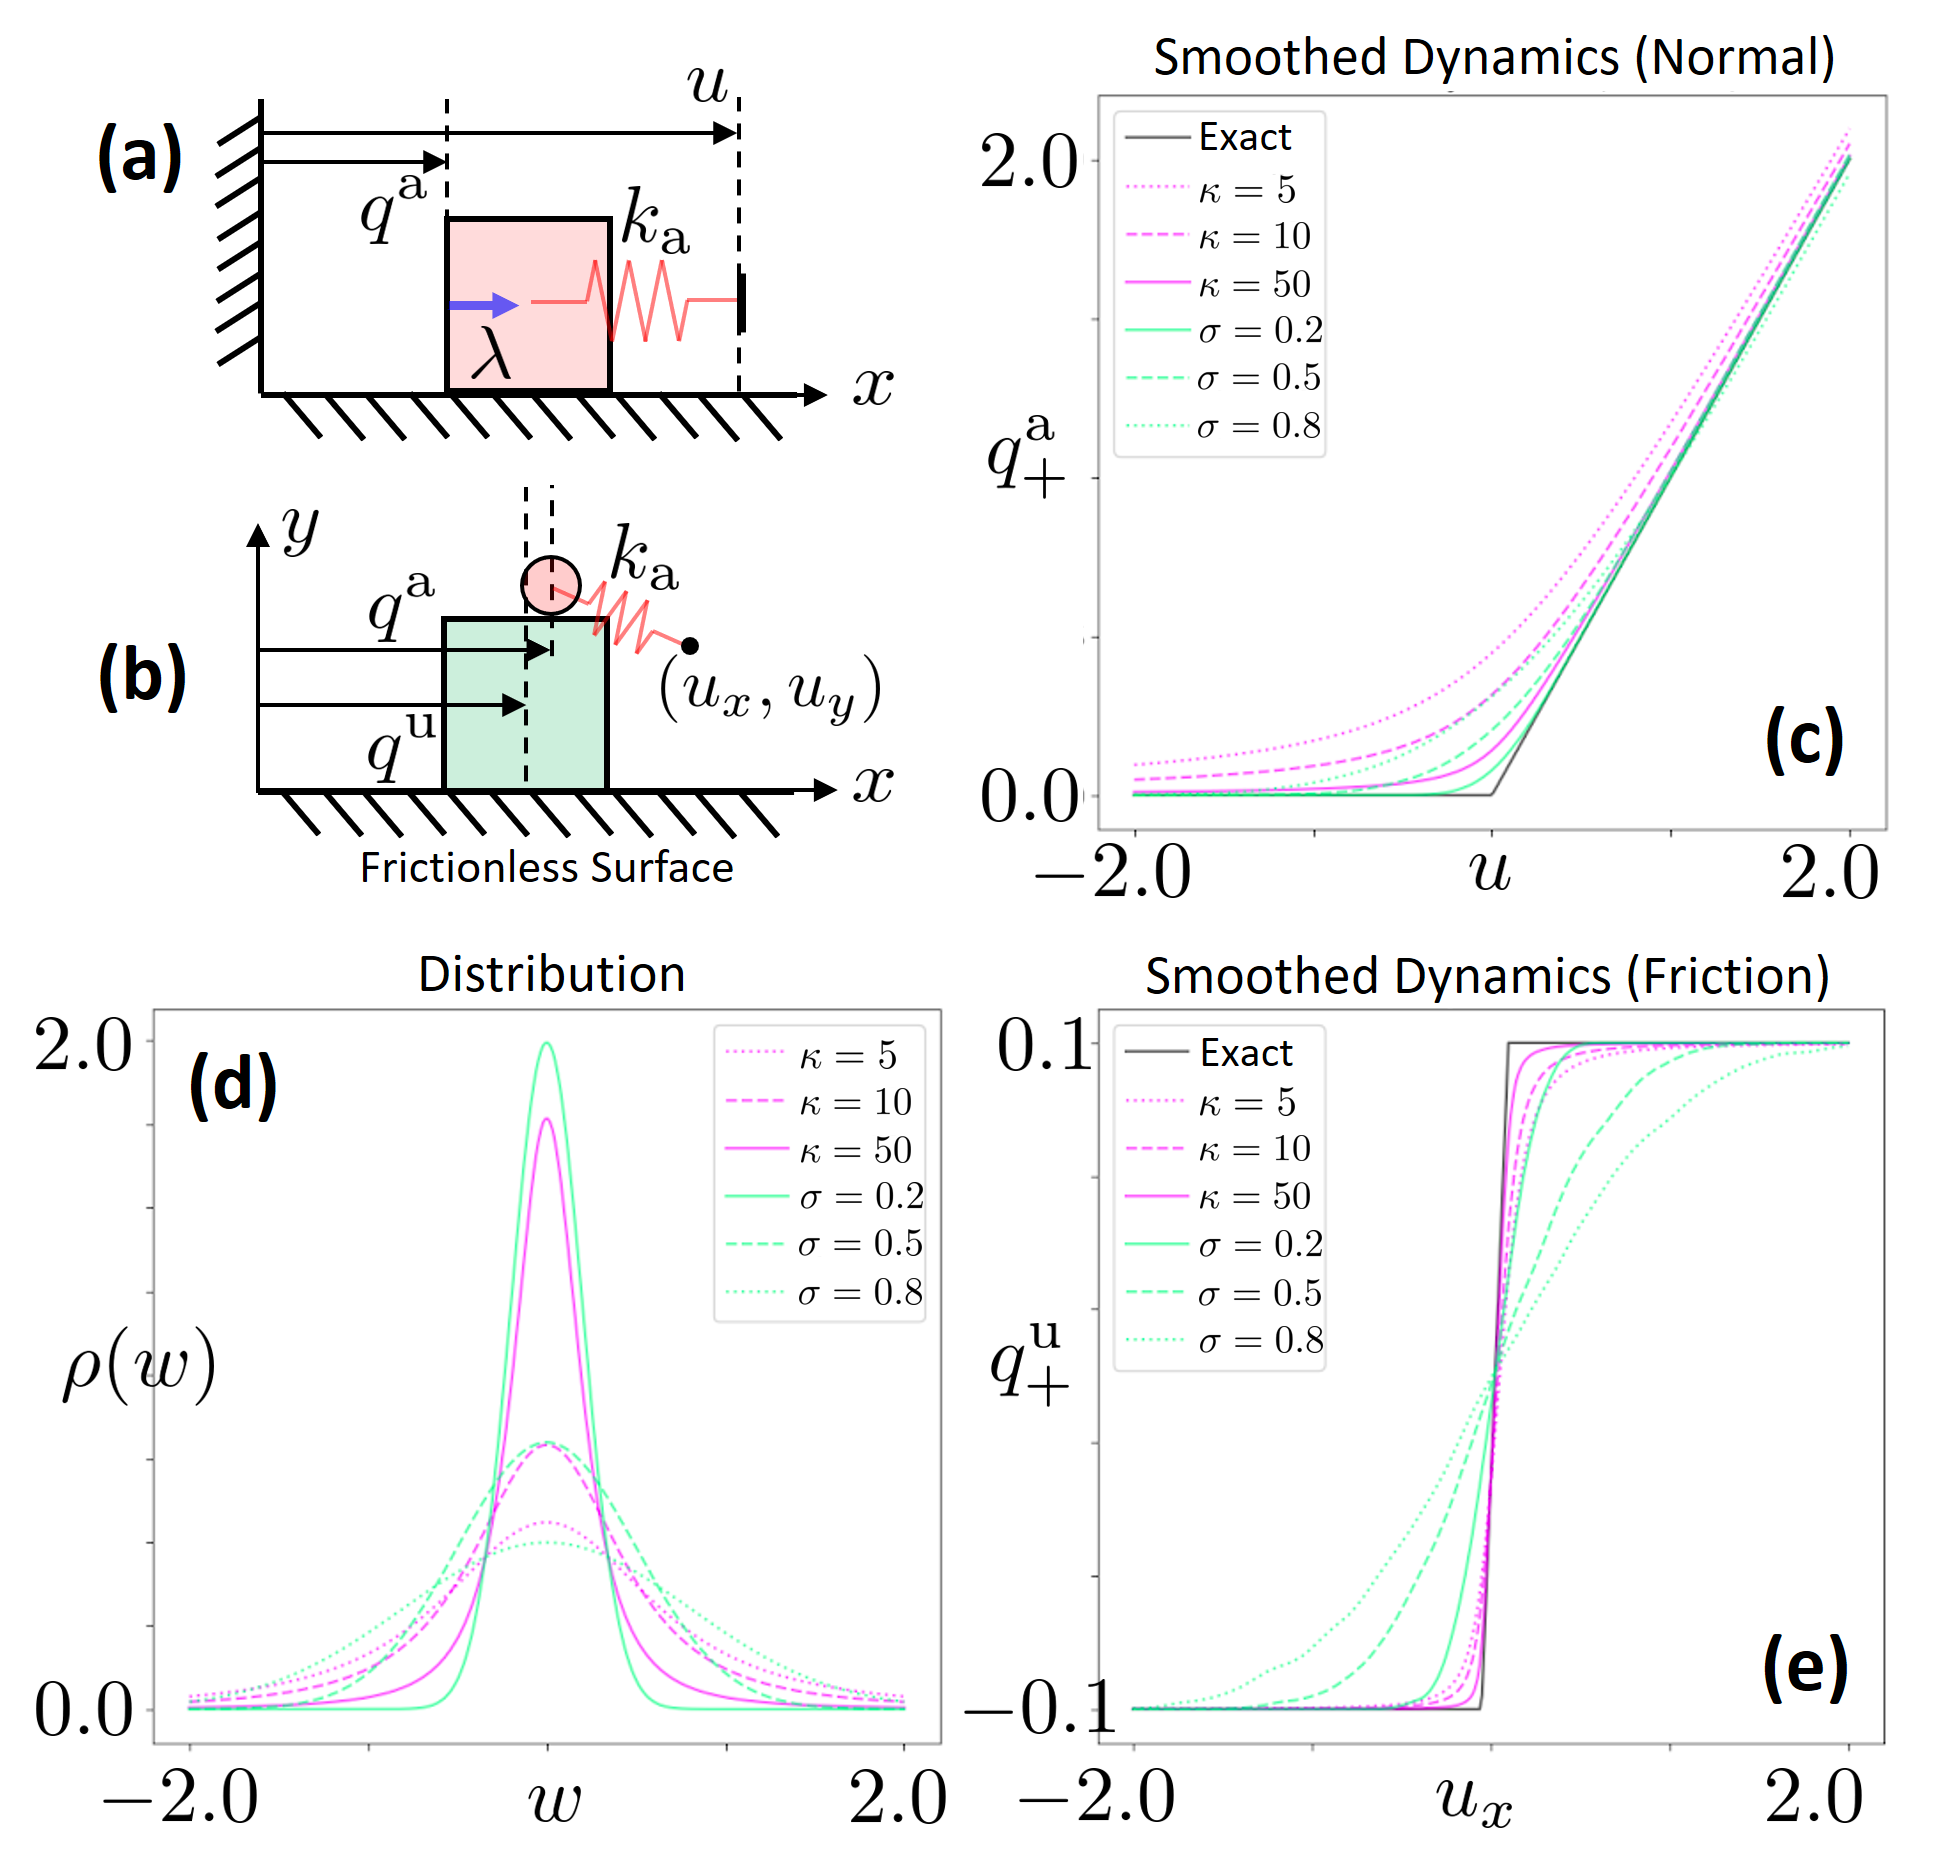
\includegraphics[width = 0.90\textwidth]{figures/02_quasi_static_dynamics/equivalence.png}
\caption{
(\textbf{a}) A system consisting of an actuated cart constrained to slide on a frictionless surface, and a wall occupying $\qa \leq 0$. The actuator has stiffness $k_\textrm{a}$.
(\textbf{b}) A system consisting of an un-actuated cart constrained to slide on a frictionless surface, and a ball actuated along both the $x$ and $y$ axes. The ball can touch the top surface of the cart with a frictional contact.
(\textbf{c}) Randomized and analytic smoothing of (a). Randomized smoothing, shown in green, is done with a Gaussian kernel with different variances $\sigma$. Analytic smoothing, shown in magenta, is done with different log-barrier weights $\kappa$. 
(\textbf{d}) Density functions of the Gaussian kernels (green) and the elliptical distributions used for analytic smoothing (magenta). 
(\textbf{e}) Randomized and analytic smoothing of (b). We plot $q^\mathrm{u}_+$ against $u_x$ for a fixed $u_y$ that is inside the cart. The linear region in the plot corresponds to sticking contact, and the flat regions to sliding.}
\label{fig:equivalence}
\end{figure}


Finally, we note that with a different smoothing scheme which relaxes complementary slackness, Howell \textit{et al.} showed a similar trend for the smoothed dynamics as the relaxation is tightened \cite[Fig. 7]{howell2022dojo}. We believe this corroborates the equivalence between analytic and randomized smoothing schemes.

